\chapter{State Of Art}\label{chap:stateOfTheArt}

\minitoc

The surveillance and control domain is a wide field of research which contains a lot of aspects such as: object tracking, object recognition, 3D mapping and area coverage among others. Our work focused specifically on the latter, i.e. finding a procedure which allows to capture a minimal number of images of a given area maximizing the coverage of the area.    
This can be achieved using a set of visual sensors. Many parameters have thus to be taken into account: size and shape of the area itself, field of view of the cameras, number of cameras (or views) to name a few. The following chapter will survey the different methods and techniques proposed in the literature to solve this problem. Keeping in mind that our  final goal is to find out a technique that works both indoor and outdoor, flexible enough to handle two scenarios: (1) a set of cameras observing simultaneously the area; (2) a single camera moving along a pre-computed path to cover the area. 

\section{Camera positioning }\label{sec:camerasPositioning}

The first step for solving the area coverage problem is the camera positioning, i.e. how to estimate an optimal viewpoint selection to ensure an acceptable coverage. It is known that an efficient camera positioning is a bottleneck in many applications, as for example in the video surveillance field \cite{11*herrera2012,12*soto2009,18*ding2012,151*zhao2013,84*xu2011}, where an efficient camera positioning is essential to monitor correctly an area.  
The following section will deal with the question of: 
\begin{itemize}
\item[-]What is a good position and orientation for a camera (i.e. a good camera pose)?
\item[-]What are the purposes of the application requiring camera positioning?

\end{itemize}
These questions have already been investigated and some solutions have been proposed in the literature. 


%\subsection{Efficient pose in a camera network: challenges and objectives}
%The first point to address is defining the pose of the camera (or set of cameras). In computer vision, the pose of a camera is composed of its position in space and orientation (or viewing direction), i.e. of 3 translations and 3 rotations in a world coordinate frame. The second point to be addressed is how to define a "good" or "optimal" camera pose(s)?\\
% To do so, it is essential to identify the purposes, tasks and priorities of the application: 
% \begin{itemize}
% \item [-] What is the final goal?
% \item [-] What are the important features for the application (e.g. to track an object, to have a high-resolution mapping, etc.)?
% \item [-] What are the shooting conditions and physical constraints?
% \end{itemize}
%   All of these aspects will have an incidence on the definition and formalization of a "good camera poses". For instance, in \cite{22*zhao2008}, the purpose is to detect tags placed on people torso which forces the camera to be positioned at a certain height with a viewing direction almost parallel to the ground; on the contrary, in \cite{146*li2011}, a camera is mounted on a UAV to monitor a vast outdoor area, which forces it to have a viewing direction almost perpendicular to the ground. 
%
%%It is important to do not confuse the finality and the objectives. For example video surveillance is the finality but the coverage of an area or the target tracking, it is required to have an efficient surveillance. The coverage is one of the objectives the most interesting and the most common about cameras positioning.
%% !!!!!!!!!
%%  The objectives are different from the finality. The objectives are the most important elements to take in consideration in order to place the set of cameras. When the finality is the global application, as for example video surveillance is the finality but the coverage of an area, the target tracking is required to have an efficient surveillance. The coverage is one of the objectives the most interesting and the most common about cameras positioning.
%%!!!!!!!!!
%%The coverage can be applied on cover each side of an object (as  in [142*]). But in most of the case the coverage is applied on area ( inside or outside). 
%
%%To have a clever and efficient cameras positioning system different aspects must be studied. First, to pose efficiently a set of cameras it is useful to know what does it mean efficient for the camera pose. To do that the objective of the cameras network have to be defined clearly. 
%
%%The objectives  vary and depending than the finality the cameras position is greatly affected.
%These two articles share the same objective, i.e. to get the best possible coverage of an area, but since the constraints and secondary objectives they must comply with are different (e.g. number of cameras, resolution, luminosity, tracking, etc.), it leads to different formulation and approach. 
%
%The next section focuses on positioning the camera to maximize viewing areas. The viewing area or coverage rate of the area is directly related to the estimated position of each camera and their orientation. To get the best coverage, it is essential to find the best pose for each camera, depending on the constraints and possible secondary goals.\\
%%(!!!! The finality and thus the secondary objective greatly, have an important influence on the camera positioning.!!!!!)
%
%Camera positioning for maximizing the coverage rate has been studied these past decades, using many different approaches. The following sub-section will provide an overview of different ways of defining the coverage drawn from the literature.
%
%%The approaches was greatly influenced by finality. In fact the finality will involve a main objective and potential some other secondary objective with their constraint. In many case the coverage maximization is the main objective but the impact of the secondary objectives are not negligible. In numerous cases, the maximization of the coverage is only the first part of the problem, hence the importance of secondary objectives.
%%The following sections are dedicated on what kind of area is covered  what is exactly the coverage with the secondary objectives  associated too.
%%%Indeed to maximize the coverage rate by optimizing the cameras position has been studied this past decade, using many different approaches. \\
%%%His approach is applicable depending on the formulation of the constraints and objectives. In numerous cases, the maximization of the coverage is only the first part of the problem, hence the importance of secondary objectives.\\
%%%The following part is focused on what kind of area is covered what is exactly called coverage and with the secondary objectives associated too.
%
%\subsection{Objective: Coverage }\label{sec:FirstObjCover}
%
%Before formalising the coverage rate to be maximised, it is necessary to define exactly what is meant by coverage: is the aim to maximise the surface area of a three-dimensional object or a 2D zone whose perimeter has been circumscribed? Is there a priori knowledge of the area to be covered (its perimeter, its bounding box, etc.) or not? Is the area to be covered homogeneous or does it contain prioritized sub-areas? 
%% Among the huge possible definition more or less restrictive the more interesting to studied is discussed: 


\begin{itemize}
%-------------------------------------------------
\item Object coverage: \\
\begin{figure}[t!]
\center
\minipage{0.75\textwidth}
   \includegraphics[width=\linewidth]{img/objectCoverFrom142.png}
  \caption{Full coverage of an object in the 3D space. The coverage is made by selecting a set of adapted waypoints. The coverage must be good enough to enable reconstruction of the 3D shape of the object without any occlusion. Result here are obtained by the method of Hoppe et al. \cite{142*hoppe2012}.}\label{fig:ObjectCover142}
  \endminipage\hfill
\end{figure}
   %The definition of a coverage can be varied this is a good example. 
   In Hoppe et al. \cite{142*hoppe2012} a good coverage is defined by the ability to have full 3D reconstruction of an object (in their 3 dimensions) with no occlusion. In this work, some prior knowledge on the object is exploited such as a rough surface description (mesh). The camera follows a trajectory "around" the object and its viewing direction is oriented towards the center of the mesh (see Figure \ref{fig:ObjectCover142}). 
  Since it is a matter of covering the 3D surface of an object, in a next-best-view strategy, this application remains too far from the one we wish to implement.  It is therefore barely applicable to our problem. \\ 
   %-------------------------------------------------
   \item Path to cover: \\
   \begin{figure}[t!]
\center
\minipage{0.75\textwidth}
   \includegraphics[width=\linewidth]{img/PathToCover[81].png}
  \caption{Illustration of "path to cover" of Nikolaidis et al. \cite{81*nikolaidis2009}. The aim is to focus on covering a road (walking path) in a small room by using only 3 cameras. }\label{fig:pathToCover81}
  \endminipage\hfill
\end{figure}
   The point here is to observe the entire trajectory commonly taken by users (car, pedestrians, …). When the area to cover is a known place, the main trajectory taken by the users can be estimated or extracted \cite{27*bodor2005}. If the area to cover is a road, for instance, then the trajectory of the driver is known \cite{14*lu2011}. In this condition, the aim is to cover the common trajectory of the user as presented in  \cite{14*lu2011,27*bodor2005,30*bodor2005,81*nikolaidis2009} (see the Figure \ref{fig:pathToCover81}). The path coverage is interesting due to the restricted area to cover: not an entire area, but only a path within a given area, that can be seen as a priority sub-area. \\
   %-------------------------------------------------
   \item Coverage priority: \\
      \begin{figure}[t!]
\center
\minipage{0.75\textwidth}
   \includegraphics[width=\linewidth]{img/MapRoI165.png}
  \caption{Map of an area to cover with crucial sub-area (region of interest), the normal sub-area  and obstacle. This map is an example of area coverage  introduced in  Jiang et al. \cite{165*jiang2010}. }\label{fig:MapRoI165}
  \endminipage\hfill
\end{figure}
   A natural way of defining the coverage in a context of insufficient number of cameras, is to define as priorities.
    In \cite{84*xu2011,165*jiang2010,171*horster2006}, some pre-defined regions are set as "priority" and called respectively "region of interest", "crucial sub-area" (see Figure \ref{fig:MapRoI165}) and "importance space weighting".  In the proposed solutions  by \cite{84*xu2011,165*jiang2010,171*horster2006}, the camera poses are in priority affected to this specific and restricted region which has the effect to neglect the other parts of the area. \\
If the environment is composed of some regions of interest, there should be also "normal" sub-areas. These "normal sub-areas" should be covered, but with lower priority. Furthermore, some  sub-areas can be defined as "no interest", which mean "not to be covered". In \cite{165*jiang2010,171*horster2006} for example, the obstacles are defined as "no interest" regions with also the consequence to  be occluding area. The idea is to keep a maximum of freedom in the camera network positioning and allow the system to handle local priority and constraints.\\
%-------------------------------------------------
\item Inside or outside area:\\ 
Another important feature to define the coverage is related to indoor/outdoor scenes. The area to cover can be typically a room with walls (indoor). Each wall must be a considered as an obstacle occluding the camera field of view,  which results in having to manage the visibility of the environment according to these obstacles and to the position of the cameras. For outdoor scenes, it is often necessary to take into account the size of the environment according to the reduced field of view of the camera. This has the effect of increasing the number of required cameras (or views) and leveraging the combinatory. 

%(also in the inside area the constraint must be the restricted posibel position of the camera (the camera must be placed on the wall for exemple))
   
\end{itemize}
  
\subsection{Additional constraints} \label{subsec:AddConst}
The common points in all the examples discussed is the aim of maximizing the coverage rate. The positioning of the cameras, and its effects on the coverage rate, is thus constrained by the application itself, the context  and the type of observed scenes.\\
%!!!!!!
%The common points in all this coverage definition is the importance to maximize it, despite the other objectives. In the examples presented the coverage was always the first and for some of them the only objective. Despite the interest for maximizing the coverage some other elements has to be taken in account to have a useful cameras position depending on the finality. 
Of course, additional constraints can have also a significant impact on the camera pose. Some of the more common constraints found in the literature are listed below:\\
\begin{itemize}
\item  The numbers of cameras: \\ In many cases,  the number of cameras used for the coverage should be minimised such as in  \cite{151*zhao2013,171*horster2006,22*zhao2008}. Limiting the number of cameras is primordial to decrease the computation time and the bandwidth. It also reduces the cost of the setup \cite{82*chrysostomou2012}. Reducing the number of cameras and optimizing their poses to get an optimal coverage are closely related tasks, not necessarily competing. Too few cameras can shrink the coverage rate by leaving black-holes in some areas of the scene. Too many cameras can result in too much overlaps and unnecessary redundancies.\\

\item Object tracking: \\
\begin{mfigures}[!]{Illustration of an covered area for tracking target. Experiment  from Ding et al. \citep{18*ding2012} }{fig:Tracking18} \centering
\mfigure{width=.65\linewidth}{img/coverageTrackingDing[18]a.png}{Initial coverage for 5 cameras dedicated to detect the  input of target.}{subfig:taget18a}
\hspace{1cm} \\
\mfigure{width=.65\linewidth}{img/coverageTrackingDing[18]b.png}{The covered area when the objective have to track several targets.}{subfig:taget18b}
\end{mfigures}	
 Constraints can arise by the objective of detecting and localising a given target \cite{18*ding2012,12*soto2009,23*liu2009,39*wu2011,40*sohrabi2000,22*zhao2008}. In such a case, camera poses must be estimated in order to track one or more targets, and possibly, be dynamically adapted. These applications very often requires an adaptation of the camera orientation (viewing direction) more than its position. This is the reason why previous work used PTZ cameras (Pan, Tilt and Zoom) as in \cite{18*ding2012,38*liu2010,12*soto2009} (see Figure \citep{18*ding2012}).
Keeping a full area covered and at the same time tracking efficiently one or more targets can be contradictory. The solution is then the result of a trade-off between coverage and tracking, as in \cite{18*ding2012} and \cite{38*liu2010}.
 In Liu et al. \cite{38*liu2010}, target tracking in a wide area is decomposed in two steps: detection and localization. Each of these steps is performed independently on each camera. Area coverage is essential to detect the targets, less for localization as the priority is, in this step, to track a target previously detected within the covered area. In the entire camera network used, one camera may be in detection mode while another is in location mode. Obviously, by adding target tracking as a constraint, camera poses and coverage are usually less efficient because of the sub set of cameras  assigned to the tracking.  \\

\item  Luminosity and environmental setup:\\ Intrinsic image quality is also a constraint that can guide area coverage. The quality of an image can result in sufficient brightness or an almost uniformly distributed histogram. In other words, the captured images must be such that they guarantee a usable signal. For example, Reddy et al. \cite{33*reddy2012} addressed first the coverage problem of a complex area and in second time,  target localization. In order to decide which target must be tracked, the quality of the image is taken into account to avoid dark areas where the target is hardly detectable. In this case, the tracking and coverage trade-off discussed in the previous paragraph is  ruled by the image quality. \\

\item  Energetic cost:
\\ Authors suggests to estimate camera positioning or path planning by minimizing a cost function that represents the energy consumption, such as in  \cite{38*liu2010,42*bulusu2001}. For instance, in Lui et al. \cite{38*liu2010}, the  objective is to cover most of an area to detect whether a target is entered in the scene or not. Secondly, the target is tracked by smart and autonomous cameras of the network. The camera set  is randomly distributed in the area and the coverage problem represents, in this case, the selection of the best cameras in order to detect the target. The selection of the cameras is estimated by both maximizing the area coverage and minimizing the energy consumption. The consumption can be consequently reduced by restricting the number of cameras set in detection mode. Indeed, the cameras are more or less power-consuming depending on the activated mode (which can be "detection", "tracking" or "sleep"). If we consider now path planning, the energy cost can be represented by the distance between two cameras or views and energy minimization is equivalent to finding the shortest path \cite{191*di2016,218*meiting2007}.  
\\
\item Multi coverage:\\
 Among the numerous possible constraints, the multi-coverage is interesting (as for example in \cite{149*mavrinac2013,151*zhao2013,152*wang2009,174*zhang2016,175*medhi2013}). It can be seen as a coverage problem where one or a few specific sub-areas must be covered by a minimum of $k$ cameras at the  same time, that is why it is also called $k$-coverage. Multi-coverage does not necessarily mean priority: a sub-area which have to be covered by several cameras is not necessarily a sub-area which must be covered in priority (more details in Section \ref{sec:zoneOfInterest}). However, mobilizing multiple cameras in a given sub-area means that fewer cameras can be used to cover the rest of the overall area. This effect can be compensated by adding cameras, if allowed. Contrarily, full-coverage of the area and k-coverage of some sub-areas will conflict and lead to a trade-off. 
 %This secondary objective in the case of limit will generate a conflict between the full coverage of the area and the $k$-coverage requirement even more with a restricted number of cameras. 
\\ 
\item  Resolution:\\ In order to keep or increase the quality of the captured images, a minimum resolution threshold or value can be fixed and used as a constraint \cite{27*bodor2005,33*reddy2012,171*horster2006,152*wang2009,43*erdem2006}. The focal length, the size of the pixel grid or the camera-target distance can serve as a measure for the resolution. However, in many applications, it is easier to adapt the distance than changing the focal length (which can be fixed and affect the calibration) or, of course, changing the size of the pixel grid. In most of the previously cited works, the distance from the target to the camera along the optical axis is therefore used as a measure for the resolution.\\
%The resolution is also model as the acceptable the depth of field.
Full coverage will tend to move the cameras at the farther distance (or higher elevation) in order to maximize the field of view. Resolution constraint will impose the cameras to be positioned at a certain range of distance or elevation. Full coverage and resolution constraint will lead to a trade-off between guaranteeing most of the area to be covered and a sufficient image resolution. The trade-off is particularly beneficial when the number of cameras is more important than the optimal need, in this case, the distance will be reduced and the resolution subsequently increased. \\
   In \cite{33*reddy2012} the problem has been formalized by using a Gaussian function in order to define the proper distance between the cameras and the target to keep an acceptable resolution for the application. \\
Here, the depth of view is used to define the range of distances. The focus point and the aperture of the camera will define the optimal distance and range in which the target is optimally focused \cite{193*fu2014}. Constraining the positioning with the depth of view can be seen somehow as a constraint on the resolution itself. 

\end{itemize}

The constraints are numerous and varied, we just introduced a few of them which seems interesting to us and related to our work. Among them, some are closely related and can be interconnected, they can even be combined as in \cite{33*reddy2012}, where the targets coverage, luminosity, resolution, are all associated to find the best camera positions maximizing the area coverage and the tracking target with good visibility condition. \\
One interesting point to study is the impact of these constraints on the full coverage itself as we have seen that they introduce a trade-off between their own particular goal and the main goal of area coverage but also between themselves. No need to say thus, that the constraints have to be chosen carefully and accordingly weighted as in any multi-objective problems. 


\subsection{Art gallery problem} \label{sec:AGP}
%Once the objectives defined the next step, is to know how to represent the problems. To do that manly 2 different class  of problems have to be studied. The first is from the geometrical problem called  the Art galery problms.

%The previous section was focus on the objectives definition as well as the finality around the sensors and cameras position

%Until now the problem was presented in term of objectives and constraint in order to be used in a concrete situation.

The Art Gallery Problem (AGP) is a theoretical and historical problem closely related to the camera positioning. The AGP is commonly cited  in the literature as a source of the problem for camera positioning (for full coverage). It is also commonly used to estimate the complexity of the task (notably due to the room shape) and  as starting point to find an appropriate solution. 
The problem of cameras positioning can be formulated as the AGP paradigm (as example \citep{44*chvatal1975,53*packer2008,149*mavrinac2013}). For these reasons, the AGP has to be well understood before going further.

%Until now the problem of coverage was studied to place cameras. The use of cameras (fix or mounted on mobile robot) are the limited field of view  and  depth field of the sensor. An interesting paradigm closely related is to use human guards  instead  of the set of cameras.  This paradigm is called the Art Gallery Problem (AGP). The AGP is an interesting  paradigm with propose some efficient solution. 

In the following sections a definition of the AGP is given with a brief history. After a more general introduction to AGP, we will describe some interesting solutions found in the literature and discuss their limitations.

%The problem of camera positioning is a tricky problem. The positioning of the set of cameras depend on many factor. To solve this problems is importatant to know more about the relat
% %finality of the camera networks and the formulation the camera pose will be affected.\\
%% Once the objectives defined ( see section \ref{sec:camerasPositioning}) the next step, is to know how to represent the problems. To do that manly 2 different paradigms have to be studied.
% The first is from the geometrical problem called the Art Gallery Problem (AGP) formulation is commonly and historically borrowed as is presents in the following section with a fast definition of the problems, the solution used and the limit of this paradigm.


	\subsubsection{Definition of the paradigm} \label{sec:AGPdef}
	\begin{figure}[t!]
\center
\minipage{0.65\textwidth}
   \includegraphics[width=\linewidth]{img/AGP3.png}
  \caption{Illustration of the AGP. The gallery is covered by  4 guards ($x_1;...;x_4$) for a polygon  composed by $n$ vertice ($v_1;...;v_n$).}\label{fig:AGP}
  \endminipage\hfill
\end{figure}
	The art gallery problem is a geometrical problem introduced by Victor Klee in 1973. The problem was the estimation of the number and the position of useful guards to cover an art gallery. 
The particularity of an art gallery is the complexity of the room shape, with many walls to place the paintings. The shape complexity of the room make the estimation of guards number even more difficult.\\
In order to formulate properly the problem, the room is assimilated as a polygon $P$, composed of $n$ vertices ($v_1; v_2;…v_n$). The vertices are linked by $n$ edges ($v_1 v_2;…; v_{n-1} v_n$) to make the shape of the Polygon $P$ (or room).

A guard $x$ is inside the room $x \in P$. A guard $x$ can cover or see any point $y \in P$ if the segment $xy$ is not intersected by one of the boundaries (walls) of the polygon $P$, in order to have $ xy \subseteq P$.
The polygon $P$ is considered as fully covered when for any position of the point $y$ in the polygon, at least one guard can see it .\\
A guard $x$ can have a $360^\circ$ field of view to cover all around him, with no depth of field limitation (except the wall obstacles). Clearly that means the guard can see and monitor the entire room from one side to the other side if there is no obstacles around to occlude its vision. For example, if the shape of the room is a triangle, quadrilateral or another simple polygon, at any position taken by one guard, this guard can monitor all the area despite the size of the art gallery (see Figure \ref{fig:AGP}). 

When the polygon is more complex, it is necessary to estimate the minimum number $g$ of guards $x$ and the position of the guards in polygon $P$. 
 The set of minimum number of guards are listed in $X$. Where $X$ contains the useful $x$ to fully cover the polygons $P$, with $g$ the minimums number of guard in order to have a set of points $X=\{x_1…x_i…. x_g\}$. So that every point $y$ in $P$  are cover by at least on guard $x$ of the set of $X$. \\
The AGP in addition to estimating the numbers of guards,  is also interested in finding the optimal position of this restricted number of guards. 
These two questions can be solved at the same time by using one of the solutions proposed.


	\subsubsection{Solutions }
	
	The advances on the AGP since its formulation in 1973 are numerous. The following paragraphs present some of the main proposals and contributions..\\
	 The first, and one of the most important, is the proof given by Chvàtal in 1975 \cite{44*chvatal1975}.  The proposed polygon must be covered by a minimum of guards, the proof of Chvàtal links the minimum number of guards $g$ to the number of vertices $n$. 
A polygon composed by $n$ vertices need in the worst case a minimum number of guards equal at $n/3$. The Chvàtal proof is based on the triangulation of the polygon. The triangulation is made based on the vertices of the polygon.\\
	 % For a polygon composed by $n$ vertices in the worst case the minimum guard necessary to cover it, is $X=n/3$.
	     The proof given by Chvàtal is also confirmed by the work of Fisk  few years later (1978). The work of Fisk is also based on triangulation and colouring node. It is probably the easiest way to understand and also give a solution to estimate the pose of each guard. It is recommended to begin by the Fisk proof before the Chvàtal one, despite the chronology order as it is recommended in \cite{219*orourke1987}. The book of O'Rourke et al. \cite{219*orourke1987} is an early work about the AGP with the formulation, proofs and advancement of the field clearly explained. \\
After the important work of Chvàtal which enable the estimation of the minimum number of guards in the worst case consequently fix a limit to the AGP. Thus, the research has been oriented toward the optimal guard positioning. The goal is to find the best algorithms to solve the AGP for all kind of polygon while reducing the complexity in time (reducing the $O(...)$).\\
%Once the proof of the minimum number in the worst case founded the objective became to find an optimal guard position for all kind of polygon in reasonable time. \\
In perspective, the work of Toussaint and Avis (in 1981) is the reference and propose a solution working in $O(n log n)$. This work has been followed and upgraded until the solution of Couto, Resend and Souza  2011 \cite{224*couto2011}. The solution  finally proposed reduce the complexity to $O(n^3)$ in the worst case. 

%It is a short overview of the AGP solution but also the solution proposed are very specific to the AGP and cannot be re-use for problem little different.

	
	\subsubsection{Limit of AGP and camera coverage relation}

The AGP can be considered as a reduction of the best camera poses estimation to maximize the coverage of a complex area. Based on the algorithms developed to solve the AGP and the strong relation between AGP and the cameras positioning (for maximum coverage problem), loigically,  some proposed algorithms have been developped. They try to extend the AGP to the  problem of camera positioning as example in \cite{221*fleishman2000,33*reddy2012,43*erdem2006}.\\
%The problem of positioning cameras for maximum coverage is quite close then the AGP. The AGP is a reduction of the camera positioning for a total coverage of a complex areas. The camera positioning is the logical continuation of AGP and once the AGP is solved , the problem can be extended as is for example show in \cite{221*fleishman2000,33*reddy2012,43*erdem2006}.
The algorithms developed for AGP cannot be applied directly on the problem of cameras positioning for maximum coverage. The main reasons are the cameras limitations such as the field of view and the depth of field (see \cite{82*chrysostomou2012,170*yabuta2008}). The cameras limitations makes  unreadable the algorithm proposed to solve the AGP; because the AGP is considering the guard with no limitations for the depth of field and field of view. Due to these differences, the geometric model of AGP may not be applicable for perspective cameras.

Also another reason that could make the AGP solution not applicable for the camera positioning is the diversity of cameras in the same system (as perspective cameras with different focal length or associate to non-perspective cameras such as omnidirectional camera).
 The AGP may have many guards, they are all interchangeable. The interchangeability is due to the guards ability (or skill) to monitor the area. Contrarily, it is possible for a camera network to have different kind of cameras with different lenses. 
Finally the  perfect assumption for the AGP formulation create important weakness when it is time to replace the guards by cameras. These weaknesses make the algorithms form AGP not adapted for our problem, as it is shown in \cite{81*nikolaidis2009,171*horster2006}.
%This weakness in the AGP formulation associate to the limited field of view  make the solution form AGP note adapted as  is showed in \cite{81*nikolaidis2009,171*horster2006}.\\Due to this limitation, the solution developed for AGP are not applicable. 

However, some part of the AGP formulation and especially some proofs are still of importance, as the proof of Chvàtal \cite{44*chvatal1975} or the NP-hard complexity proof. 
In fact, the AGP formulation as a NP-hard problems is available in the book of O’Rourke section 9.2\cite{219*orourke1987}. NP-hard means that the problem cannot be solved in a deterministic manner with a reasonable time. 
In order to demonstrate the AGP  NP-hard, the first part to be considered is the reduction of the  problem to another well-known problem for this complexity. The relation is made by reducing the AGP with a polygon composed by  holes to another standard problem: in the demonstration, the 3SAT is used to be exact. 
The 3SAT is a restriction of the SAT problem with atleast 3 literals in each clause (example of  1 clause with 3 literals $(x\lor \neg y \land z)$) , the SAT has to satisfy a boolean expression written with only AND $\land$, OR $\lor$, NOT $\neg$) by assigning the appropriate value to the variable of the boolean expression (True or False).\\
Once the AGP is reduced to 3SAT (see \citep{227*tovey1984}) and because 3SAT is an NP-complete problem, the AGP is  also considered as NP-complete or  NP-hard but under conditions:   the room have to be composed of holes. In addition, another work of Lee and Lin 1986 proved the complexity of AGP \textit{without hole} also by reducing the AGP to another well known problem (for more explication see the book of O’Rourke  section 9.3 \cite{219*orourke1987}).
Despite the limit of AGP, numerous articles are based on it to formulate the problem as in \cite{43*erdem2006,53*packer2008}. For example in \cite{43*erdem2006} a similar approach to AGP is used in order to estimate the occluded regions. 
As explained earlier the cameras positioning can be reduced as an AGP \cite{53*packer2008}, notably by removing most of the constraints due to the camera properties (as depth of field and field of views). 

In the literature numerous articles uses the AGP as reference to explain the complexity of the problem of camera positioning, for example \cite{26*moeini,44*chvatal1975,149*mavrinac2013,151*zhao2013}. The problem of camera positioning for maximum coverage is at least NP-hard or NP-complete as stated above. 
The complexity of the problem will have an impact on the solution tested  to solve and optimize it.\\
Another impact of AGP in the problem of camera positioning is the shape of the rooms. In \cite{170*yabuta2008,171*horster2006,33*reddy2012,43*erdem2006}, the shape of the room to cover is similar to the definition of an art gallery (in AGP). The art gallery room is a complex polygon composed by many vertices which may occlude the view (as explain in Section \ref{sec:AGPdef} and as in the Figure \ref{fig:AGP}). This phenomenon can be imputed to the link made between the number of vertices and the effective number of guards to cover it. 
In addition, the occlusion formulation made for the AGP is commonly used.
The occlusion in AGP is defined  by  a segment $xy \not\subset P$   where $x \in P$ is the guard position $y \in P$ is a point in the room $P$. 
Moreover the usage of a complex room inspired by AGP is therefore a good choice in order to verify the effectiveness of the algorithms developed for the cameras positioning in a complex environment.
%The complexity of this problem is also an important factor which makes the relation of camera positioning and AGP. \\


The AGP can be interpreted as the  historical source of the cameras positioning and give a beginning of a solution about the problem, its formulation and its complexity. Despite that, the AGP is not the only source to refer about the cameras positioning for maximizing the coverage. Some clue and algorithms can be found in other related fields. 


\subsection{Wireless sensor network }\label{sec:WSNstateOfArt}

The Wireless Sensor Network (WSN) can be, as the AGP, considered like an inspiration for the problem of cameras positioning to maximize the coverage. The WSN is an active field of research related in many aspects to camera positioning. These sections are focused on the WSN and its relation with the cameras positioning.\\ 

\textbf{What is the Wireless Sensor Network (WSN)? }

 The WSN is a distributed network of sensors or in some cases actuators. It can also be called WSAN (Wireless Sensors and Actuators Network). Each sensor of the network acts as a relay for the information to the rest of the network.  
The sensors are at the same time the nodes and the relay for the network. The node has the purpose to transmit the information to the other node. 
The information can be centralized or not :
\begin{itemize}
\item When the system is centralized, the information has to be transmitted node to node up to the centralized agent. The computation and the decision about the network is taken by the centralized agent before the transmission back to the node. 
\item Otherwise, the node is the sensor, collects information and decides to communicate with the other nodes depending on the situation (example when the target is detected in their field). The node  manage itself or with its neighborhood the information and computation before reacting in consequences. 

\end{itemize}
 
The information collected by the sensors are vast depending on the final application and the capacities of the sensors ability. 
The WSN is used in different fields for various applications such as Telecom with antenna positioning \cite{59*wang2008}, military surveillance field \cite{38*liu2010,101*topcuoglu2009}, airport surveillance \cite{37*ma2012}, video surveillance and tracking \cite{38*liu2010}, environmental monitoring \cite{42*bulusu2001} etc. 
Consequently, the sensors is able to collect numerous type of informations depending the need: temperature, movements, images, song and also some  actuator can be used as radio frequency for example.\\
 The applications of WSN are wide, especially since the WSN can be exploited in many applicative fields. The WSN tries to optimize a network of sensors in different aspects, for example \cite{39*wu2011} focus on an adapted architecture efficient enough for data transfer (here the data are images) ; otherwise in \cite{40*sohrabi2000} the WSN are dedicated to adapt the network around static nodes and energetic resources in order to keep the network connected.  \\
In our case, the most interesting aspect of the WSN, is the coverage of an area with constraints.
 The other disciplines of the WSN such as the network optimization will not be addressed in the following document. Only the problem of coverage is studied: the other discipline are not considered as the first or main objective but can be some secondary objectives after the problem of coverage which has to be taken in account for the optimization. 

\subsubsection{Sensor at 360}
%
	\begin{figure}[t!]
	\center
\minipage{0.55\textwidth}
   \includegraphics[width=\linewidth]{img/WsnSensor1.png}
  \caption{An omnidirectional sensor centred on $x$, with a radius $r$ for the range.}\label{fig:WsnSensor1}
  \endminipage\hfill
\end{figure}

	

The WSN refers commonly to sensors or actuators  with no restriction in the view angle, considered to own a $360^\circ$ field of view. The sensor field of view can be represented  as a circle in a 2D plan like in \cite{200*kulkarni2011, 174*zhang2016,150*chakrabarty2002} (as illustrated in the Figure \ref{fig:WsnSensor1}) and in some case a spherical shape for the 3D environment examples in \cite{175*medhi2013,59*wang2008}.  \\
Each sensor have a position $x$ in the area and a power range. From the sensor power,  the radius $r$ of the circle is deduced from $x$ the center (see Figure \ref{fig:WsnSensor1}). This circle gives the area covered by a sensor in the simplest case. 
The simplest case correspond to a flat area without any obstacle as shown in \cite{200*kulkarni2011,174*zhang2016} (see the Figure \ref{fig:WsnSensorNet}).  
In addition, more complex solutions can be used. A more complex solution but also more realistic is the one proposed by Wang et al. \cite{59*wang2008} where the obstacles reflief is taken into account in the process.
In Zhang et al. \cite{174*zhang2016}, more complex model have been developed where, despite of a flat ground without obstacle, each sensor is represented by a perception radius and a communication radius. The communication radius a bit bigger than the perception radius. These two radius with the same center corresponds, first to area covered by one antenna (sensors for the perception) and the second radius to the distance of emission/reception of the data (actuators for the transition).  To have an efficient coverage of the area, the antennas must be placed in order to have connections with other antenna but without too much overlap of the perceptive field.\\

The solution proposed in order to optimize the positioning of the WSN for a circular sensors can be numerous. Mostly two different ways are applied for the sensor which have circular angle of view or spherical.\\
\begin{figure}[t!]
	\center
\minipage{0.65\textwidth}
   \includegraphics[width=\linewidth]{img/sensorWSN3.png}
  \caption{Illustration fo a  simple wireless sensor network with omnidirectional sensor centred on $x$, with a radius $r$.}\label{fig:WsnSensorNet}
  \endminipage\hfill
\end{figure}
\begin{itemize}


\item	The first solution use a heuristic based on geometry construction as in  Medhi et al. \cite{175*medhi2013}. This approach gives a good coverage solution but is usually greedy and can be quickly limited due to an important number of sensors required. Moreover if some external constraints are added.  For example in Zhang et al. \cite{174*zhang2016} the greedy solution was tested and optimized by using a "partition and shifting" strategy in order to upgrade the result.
The limit of this solution is this greediness of the process. In addition, it is not applicable to the problem of cameras positioning due to the reduced field of view of a camera.  \\
\item	The second solution intends to find an efficient and quick solution to optimize initial random position, for each sensor of the network.  
This solution includes many different families of algorithms focused on optimization.
Among the family of algorithms, the evolutionary algorithms (disused in detailed in Chapter \ref{chap:EA}) is commonly used as in \cite{200*kulkarni2011,59*wang2008}, and \cite{150*chakrabarty2002}. \\
These solutions propose to optimize the position in order to maximize the coverage depending on constraints. The method of optimization have to be adapted to the problem. 
In Chakrabarty et al. \cite{150*chakrabarty2002} the integer linear programming  is chosen in order to maximize the coverage with two types of sensor. One standard with a smaller area coverage but with a smaller cost ($100m$ radius for 150\$) and the other sensors can cover a wider region ( $200m$  radius for 200\$) . The objective is to cover the region while reducing the financial cost using integer linear programming adapted to the problem of coverage optimization. \\
In \cite{59*wang2008} and \cite{200*kulkarni2011} the solutions proposed are based on two different evolutionary algorithms in order to optimize the sensors positioning. 
In Kulkarni et al. \cite{200*kulkarni2011} the camera positioning with a multi-coverage is solved by using an evolutionary algorithm called Particles Swarm Optimization (PSO). The objective is to optimize the position of the sensor in order to have an efficient coverage of the area and also enough redundancy to keep the network workable if one or few sensors fail. In Wang et al. \cite{59*wang2008}, an evolutionary algorithms is also used to optimize the position of antennas. The objectives in this paper is to give the best coverage of an area with taking in count the relief of the area. The relief make the coverage estimation of each sensor even more complex and costly in terms of time computation. The genetic algorithm is used in order to find quickly a position for each antenna of the network. 
\end{itemize}

Among the solutions proposed, the second, based on optimization of a set of sensors position  depending on the constraints is the most intersting and the more flexible to the addition of new additional constraints (and secondary objectives). \\
The following sections is dedicated to validate if these solutions are applicable to the problem of positioning a camera set  despite the camera constraints.
%The aim is to see up to what point and if it is applicable to the problem of cameras network positioning.  

	\subsubsection{Visual sensors}
	
	\begin{figure}[t!]
	\center
\minipage{0.65\textwidth}
   \includegraphics[width=\linewidth]{img/coverage[165].png}
  \caption{Illustration of  the  area coverage with visual sensors. The area  is covered at 47\%. Experiment form Jiang et al. \citep{165*jiang2010} }\label{fig:Coverage165}
  \endminipage\hfill
\end{figure}
	
%Logically, the result obtained with the Omni-directional sensors are interesting.
% These methods of  omni-directional sensors must be applied to the problem with even more constraints and objectives for the positioning of Visual Sensor Network (VSN).
Positioning visual sensor can be, by numerous aspect, closely related to AGP and the WSN.
These previous methods must be even more constrained to enable the usage of a perspective camera due to the limited field of view.  
Visual sensors embed different types of cameras and  modalities, even though the most commonly used and studied is the perspective camera such  as in \citep{149*mavrinac2013,174*zhang2016,193*fu2014,42*bulusu2001,165*jiang2010} (see Figure \ref{fig:Coverage165}). 
%The term of  visual sensor contains several types of cameras with several constraints and properties. Despite these several types of cameras, the more commonly used and studied is the perspective camera ()
  %In fact, the visual sensor or camera have a limited depth of field but also a limited field of view. 
  These constraints makes the camera positioning relatively more complex, as it is necessary from AGP point of view (see Section \ref{sec:AGP}) to pass from guards to cameras.
   Contrarily, WSN already takes into account the  limited depth of field  which  makes it more  suited  to perspective cameras.
   
Heuristic-based solutions applied to omnidirectional sensors cannot be deployed for perspective cameras (which would require the definition of new heuristics and not only an adaptation), however optimization-based solutions can be adapted to it by only adjusting the constraints. The following sections will discuss such kind of techniques and solutions. 
 
 
 
 %but also the problem is formalized as optimization problems with some solutions based on optimization and meta-heuristic. This way to present the problem is appear as the more suitable to add constraint and secondary objectives. Also the solution and the formulation for the problem of VSN are mostly the same then the problems of cameras positioning and is discussed in the following parts  \\
  

	\section{Solutions not based on evolutionary methods}\label{sec:NonEAmethod}
	
The algorithms used to estimate the pose of a camera set  in order to maximize the coverage are numerous. Two main classes can be defined: the first one, which is called "constructive", is a step-by-step positioning of the cameras, one after the other; the second one comprises the optimization-based solutions. Most of these approaches fall under either the AGP paradigm or the WSN paradigm, or even a combination of both.\\

\subsection{The constructive solution}

The camera positioning can be done by a progressive construction, i.e. a deterministic method is applied to locate iteratively one camera after another or to adjust their positions based on an initial set-up.\\
For instance, in Liu et al. \cite{38*liu2010}, a constructive solution is applied in order to select the smart cameras of a network. Each smart camera is  a node of the network transmitting information and images. The smart cameras are fully autonomous in terms of energy and decision-making (no central master). 
The nodes can be set to three different modes:
\begin{itemize}
\item[-] Sleepy mode. It is used in order to save the energy consumption. The camera is turned off which means no computation tasks are performed but the network is listened at regular intervals to wait for the wake-up call.   \\

\item[-] Detection mode. In this mode, the camera is turned on, but with a low frame rate. Just a few computations are done to detect if a target enters the field of view. Some information may be transmitted by the network. This mode consumes more energy than the previous one, however the smart cameras can still stay in this mode for a long time.\\

\item[-] Tracking mode. This mode is the more active, thus the more energy consumer. The camera is turned on with a high frame rate and numerous computations are done to track and localize the targets. Also more informations have to be transmitted by and to the network. Localizing and tracking a target is a collaborative and distributed task between several smart cameras of the network.  
\end{itemize}
The objectives in \cite{38*liu2010} are multiple, depending on the state of the cameras. The most interesting for our application is to keep under control the area as long as possible, for target detection. Numerous smart cameras are randomly distributed in the area (as an air-drop in a battlefield) and the aim would be to select the minimal number of cameras which allows to maximize the coverage by setting them in detection mode. The solution proposed by Liu et al. in \cite{38*liu2010} rely in the usage of a constructive algorithm. The network of cameras self-organize itself after a "discussion". Also each smart camera is able to estimate precisely its own localization: this is a key information to select the cameras to set up in detection mode. The solution proposed is directly inspired by the distributed network communication protocol. \\
All the sensors are in sleepy mode at first. The cameras wakes up regularly and send a call at the neighborhood: if they receive no reply, this means no other camera is awake around and the camera switches to the detection mode. If a few replies are received (the threshold must be set up), this means that the required density of the camera around is not reached yet. Thus the camera switches or keeps on detection mode. Otherwise the camera switches back on sleepy mode until the next wake-up (in this case, the density threshold is reached). Each smart camera follows this protocol but the sleeping time is inherent to each camera to avoid they all wake-up simultaneously. After a certain time, the network is well enough organized to cover the area in detection mode. The area is considered covered when the density of camera is good enough. \\
 The method introduced by Liu et al. in \cite{38*liu2010} is efficient. The solution proposed has the advantage to work in wide areas and to be dynamic. For example, if a camera does not have any more power, the network will self-reconfigure. But it suffers also from some drawbacks. First, it requires a high number of cameras with some of them being "useless" because of the sleepy mode. Also this method is really dependent on the network communication and the capability to localize accurately each camera. Finally, extracting a sub-set of cameras among a randomly distributed network (in which the cameras are static) does not give a sufficiently accurate localization to allow a appropriately satisfying coverage (see Figure \ref{fig:Coverage38}). 
	\begin{figure}[t!]
	\center
\minipage{0.65\textwidth}
   \includegraphics[width=\linewidth]{img/From38Liu.png}
  \caption{Illustration of  the  area coverage with smart cameras and a target tracking objective. The smart cameras can be in 3 modes (sleepy, detecting , locating). Experiment made in Liu et al. \citep{38*liu2010}}\label{fig:Coverage38}
  \endminipage\hfill
\end{figure} 

Another cameras pose estimation by construction is proposed by Höster et al. \cite{171*horster2006}.
The solutions proposed is based on a greedy search heuristic. The objective is to find the positions and orientations for a camera set  with a fixed pan, in the environment inspired by the AGP. \\
In \cite{171*horster2006}, a first greedy search solution has been presented before another algorithm which extend the greedy solution. The algorithms developed in \cite{171*horster2006} is called Dual Sampling.\\
The dual sampling is an incremental method. 
First step, is the initialization of the position for all the cameras. A random initialization for the position and the orientation must be appropriate.  \\
Second step, is the selection of one point of the area that is not covered yet. The area is discretized by several points, with each point that must be covered by at least one camera. Around the selected point, several positions and orientations are tested for the cameras nearby. The possible position are obtained by sampling the area around the point to cover. Finally the best cameras position and orientation is kept. The best cameras positions and orientations depends on the number of other points globally covered in the area. 
The second step is repeated and the set of uncovered control points are reduced at each iteration. This procedure is applied until the stopping criterion is reached. Which means, enough points of the area are covered. \\
The constructive solution have some inconvenient, notably in terms of efficiency. Indeed this solution is limited by the number of cameras and size of the area due to the exponential difficulty. %In fact, bigger area mean more point and more camera mean more position and orientation to test at each iteration.

In Nikolaidis et al. \cite{81*nikolaidis2009}, the cameras placement is studied to cover a basic mobile robot trajectory.
The trajectory of the mobile robot is modelled as the regions of interest, with a gradually decreasing interested from the trajectory center.\\
  The solution applied in \cite{81*nikolaidis2009} lie in performing a local optimization one camera after another with the “steepest decent method" (related to  the gradient decent). If this local optimization gives a better solution, the network of camera is modified, otherwise, the cameras stays at the same place. This operation is repeated until the convergent arrangement is obtained or if no more upgrade can be found. The result presented in the experiment done by Nikolaidis in  \cite{81*nikolaidis2009} are intresting despite the simplicity of the area and the very small amount of cameras used (maximum four). The main limitation is due to the number of steps required to optimize independently each camera of the network. Also a multitude of local optimization is not obviously the same or better than a global optimization.

Ma et al. \cite{37*ma2012} proposed a solution for the problem of finding the minimum camera barrier coverage. 
The objective of the camera barrier is to cover only the boundary of an area, to be able to detect target intrusion  within the perimeter. 
The perimeter is relatively wide and can be considered at some point as an area to cover composed by a big hole in its center.\\
 The region to cover is divided into numerous sub-regions which are inter-connected. Each sub-region must be “full-view covered”. The full-view covering is defined as follows: regardless of the direction in which the target is moving, there must be a camera to detect his/her face - in the case, for example, of a video surveillance of a building.\\
The proposed solution is based on constructive solution with adapted heuristic. The heuristic used is presented in details in \cite{37*ma2012}. The global idea is to divide the perimeter in different sub-regions and apply the method proposed to have a full-view coverage at each sub-region. 
Dividing the region into sub-regions allows to speed up the processing time of the algorithm.\\
This solution is well suited  for visual coverage of the perimeter  but much less for coverage of an entire surface, which is the case we would like to address.  
%Thesolution proposed though this efficiency in the case of barrier coverage is not rely appropriate for vast coverage area.
 The first limitation is the number of cameras used to cover the area. However, this method require a large number of cameras, this definition implies many overlaps to have the full view coverage.

The previous solutions and algorithms presented in \cite{38*liu2010, 37*ma2012,81*nikolaidis2009,171*horster2006} are based on constructive methods for the camera placement and their local optimization. The positioning of the camera network  is carried  out camera per camera successively and iteratively.  %is individually located  depending on the network with an iterative process.
% The iterative process has to chose the best position for each camera of the set. 
This method has some consequence, notably, the fast increasing number of iterations required to have a sufficiently accurate solution. The time complexity is even more problematic while increasing the size of the area and even more while  increasing the number of cameras. Also these solutions are extremely dependent on the formulation and the constraints and cannot be easily adapted to other closely related problems (new constraints  or modified objectives). The poor adaptability   of the method is mostly due to the  use of heuristics designed for very specific problems. 

\subsection{Linear programming optimization and limits}
	Different methods of linear optimization were applied and tested in the literature. Linear optimization, when based  on  a  judiciously  adapted  formulation, can be very effective on small convex areas  which remains very restrictive %In some cases, due to a well-adapted formulation, a specific shape of the area or cameras number the linear optimisation is efficient. 
 This is the reason why linear optimization is often used for comparison with more flexible and efficient methods more as a research contribution (as in \cite{,151*zhao2013,82*chrysostomou2012}). 
%The linear optimisation  has been  tested in the literature in order to have a reference point to compare the other more appropriate solutions (as example \cite{,151*zhao2013,82*chrysostomou2012}).

	%The linear optimisation has been tested to have initial result in order to have a reference point before to develop other solution .  
%	The reason ofIn some other case the method was studied but finally rejected du to this fast limitation 
	 %The linear optimisation  is finally rejected due to this fast limitation.  Indeed the linear optimization can be quickly in difficulty due to the fast increasing complexity of the problem and in many case be locked in local minima. 
	 The following section will show the interest and the limitation of the linear programming based on examples from the literature.

%%\textbf{!!!!!! partie manguante sur l'utilation des methode linear  !!!!!(voir path planning)}
% non linear	 141*akbarzadeh2013,33*reddy2012 
	 \subsubsection{Linear programming}
	 The linear programming is applicable for the linear and convex problems in order to minimize a linear and convex cost function.\\
The paper of  Erdem et al. \cite{43*erdem2006} is based on AGP and  WSN by proposing a fusion of the two paradigms. Some modifications have been proposed to impose  a  field of view limitation which is not initially included in the AGP. 
 %take into account the field of view limitation.
  On interesting aspect is how some camera properties have been modelized to fit with the problem of AGP.  \\
In \cite{43*erdem2006}, PTZ cameras are set up  with the task of zooming,  50mm or 35mm. The area to cover  and  the cameras parameters are discretized.
The solution proposed being usable  using an omnidirectional camera or considering a PTZ as an omnidirectional camera while  performing an efficient angular sweeping. The omnidirectional cameras are simulated by PTZ camera with a non-continue zoom  as in the experimentation proposed in \cite{43*erdem2006}. Where the PTZ can have two focal lengths at 50mm and  35mm. 
Finally the solution proposed is to discretize the area to cover and also the different possible parameters for a camera (as: localization, orientation, focal...). In order to have a combinatorial formulation of the problem. Thanks to this formulation close to the Binary Integer Programming (BIP) and the application of a well-known method “Branch and Bound” in order to optimize the cameras placement.  \\
This solution  proposes a  good  coverage with the minimum of cameras in a reasonable time. The main limit of the solution is due to  the  use of omnidirectional or simile omnidirectional cameras.% until, the  number of location sample, the numbers of cameras, and the number of parameters possible for the camera stay relatively  reduced.  \\

Zhao  et al. \cite{22*zhao2008} intended to find the optimal position for a camera set  in order to maximize an indoor area coverage (similar to an art gallery room). The coverage of an indoor area is not the main objective, which is tag detection in the scene. 
The solution proposed for the coverage is to adapt the number of points of interest which must be covered by the camera depending on the coverage rate. \\
The area is discretized as a grid.  The grid is composed of smartly selected points. Each point of the grid represents a potential location of the target.
Cameras are located in a few fixed positions on the walls of the room. 
% number of possible position for the camera (the boundary of the room) are defined.
The adapted grid and the restricted  camera positioning are used to limit the size of the search space (as a number of possible solution). Thanks to this limited search space a linear optimization with the BIP can be used. \\
BIP is a popular method that has been widely used such as in \cite{22*zhao2008,43*erdem2006}. In \cite{22*zhao2008}, the solution proposed is using BIP formulation, the smart sampling of the grid and branch and bound from LP\_solve libraries to optimize the camera poses.

% A Similar method is used in \cite{27*bodor2005} to find the position and orientation of a set of cameras. The goal of this paper is to find the appropriate position with maximize the resolution for a set of cameras dedicate to do tracking. The position is determined depending on a set of standard pedestrian trajectories. The camera pose try to maximize the given trajectory to have the best resolution and the entire coverage. \\
%The problem is also formulate in order to apply a linear well-known algorithm. In this case the branch and bound is applied.  

\subsubsection{Limitation of linear method}
The methods of linear optimization were applied and tested to solve the problem of camera positioning for maximum coverage. In some cases, due to a well-adapted formulation or a restricted area and camera number, this solution is efficient enough. In some other cases, the methods were studied, but finally rejected because of their relatively bad performances when the number of cameras is high, or the room size and so on, as example \cite{141*akbarzadeh2013,151*zhao2013,82*chrysostomou2012}). Indeed, linear optimization is quickly challenged, or even failed, when the complexity of the problem increases (the solution can then converge to a local minimum). 

Wang et al. \cite{181*wang2017} proposes a solution with an atypical problem formulation. The solution proposed in \cite{181*wang2017} will modulate the point sampling with respect to the room shape complexity (more points on the boundaries or obstacles and less on the center or "flat" areas). The idea is to have an area discretized with precision by using the minimum number of points. 
                               
The main advantage of this solution is to propose an area representation with enough sharpness and a minimum number of points. Less points to describe the area to cover mean also a gain in time efficiency  during the camera poses estimation (solving the cost function is faster).
Despite this interesting solution, the results presented in the experiments does not appear to be conclusive.  

The main problem of the linear optimization appears when the problem becomes too complex. The complexity can come from the formulation and also from the additional constraints. But, in many cases, the increased complexity comes from the increased size of the search space. In practice, when the objective is to place a larger number of cameras or when the number of positions and orientations is too large, linear optimization may not work. 
	 
	
\subsection{Game theory} 
	 
Among all the possible solutions, an atypical method is to apply the game theory \cite{19*li2013}. The game theory is used to optimize the viewing direction of the cameras as in \cite{12*soto2009,18*ding2012,19*li2013,25*song2008}. These articles are based on game theory to find an equilibrium (also named Nash equilibrium) between two contradictory objectives. The objectives are, on one hand, to maximize the camera resolution and, on the other hand, to perform a multi-target tracking.

Soto et al. \cite{12*soto2009} proposed a network containing a dozen of PTZ cameras. That means the position of the cameras are fixed and the solution proposed found the best orientations with the appropriate focal length to track most of the targets.  \\
 To do so, the camera are smart enough to communicate with the close neighbors and adapt the pan, tilt and zoom depending on the objectives.
The objectives have been defined by an utility function (or local cost function). The goal is to track most of the targets as possible with the better resolution. The cameras have reached the goal when they obtained a desired image resolution for all the visible targets.
 The multi-target issue can seem far from the coverage maximization we are interested in. But the number of targets may be higher than the number of cameras. The higher number of targets push the camera tracking to be an interesting solution to maximize the coverage of an area. In this case, the quality of the coverage will also depend on the number of targets and the importance of the resolution constraint.  \\
	 In \cite{18*ding2012} and \cite{25*song2008}, different experiments have been proposed with a number of targets which increases progressively.\\
	  Furthermore, the decentralized solution (as proposed in \cite{25*song2008} and \cite{18*ding2012}) is more adapted to prevent the security issues such as wrong transmission and interceptions by hostile opponents.  Obviously the security and the integrity of the system are primordial key points in the surveillance application. %The decentralization of the system allow to process directly the information.  %(or more exactly in this case for tracking)
To have the decentralized system the cameras must have some autonomy. \\
In the experiment proposed in \cite{12*soto2009} and \cite{18*ding2012,25*song2008}, each camera is smart enough to have its own tracking and control module. Also the cameras are able to communicate with each other, until a consensus is reached. The consensus is found when a Nash equilibrium is found between the two contradictory objectives. In this case it is a win win situation for both objectives.\\
So the objectives are not independently optimized, moreover the solution proposed have to optimize the objectives  simultaneously in order to reach a consensus. The consensus is  then also reached when it is no more possible to upgrade one of the objectives without downgrading the other one.\\
  In the experiments of \cite{18*ding2012,25*song2008}, the consensus is found thanks to the cameras communications. The cameras communications have to maximize numbers of target covered with the higher resolution.
 The experiment is based on numerous targets moving freely in the area. Also in \cite{18*ding2012}, one of the target must be covered in priority with a high resolution. This has an impact on the other camera positions.
 The results of the experiment as shown in Figure \ref{fig:CoverageFrom18} from \cite{18*ding2012} shows a really efficient global coverage with almost all the targets covered at every time-frame despite the movements of the targets. \\
 The advantage of these solutions is the suitable result and  the dynamic reconfiguration of the system for a reasonable size of the area and a decentralized computations. The decentralized computation of the system allows to process directly the information on each camera.\\ 
Otherwise this method has some limitations, as shown in the experiment, the area is relatively restricted and numerous cameras with a fixed position are needed. A consequence is that a sufficient and significant overlap is required. 
%The consequences is the quantity of overlap, relatively important.
 In this case the number of sensors is not perfectly optimized to cover the area. Moreover to use properly this method for maximum coverage, it requires a large number of simulated targets in the region to observe (there should be more targets than cameras).  Finally this solution is more adapted for a self-reorganization for a set of PTZ cameras.

\begin{figure}[t!]
\center
\minipage{0.905\textwidth}
   \includegraphics[width=\linewidth]{img/CoverageFrom18.png}
  \caption{Result of coverd area after the game theory optimization. The objective of the game therory is to maximize the tracking and the resolution. The results shown are from the experiment made in \cite{18*ding2012}.The images are representing the iterative sequences for the targets tracking and maximized resolution.}\label{fig:CoverageFrom18}\endminipage\hfill
\end{figure}
	
	%%%%%%%%%%%table sum up%%%%%%%%%%%%%%%%%%%%%%%%%%
	% Please add the following required packages to your document preamble:
% \usepackage{booktabs}
% \usepackage[table,xcdraw]{xcolor}
% If you use beamer only pass "xcolor=table" option, i.e. \documentclass[xcolor=table]{beamer}
%\begin{landscape}
%
%	\begin{table}[]
%\centering
%\caption{Sum up articles.}
%\label{my-label}
%\begin{tabular}{@{}lp{2.6cm}lllp{1.6cm}p{1.6cm}llp{1.3cm}p{1.3cm}p{1.65cm}p{1.6cm}p{1.3cm}p{1.3cm}p{1.4cm}@{}}
%\toprule
%\multicolumn{1}{|l|}{\textbf{ref}}               & \multicolumn{1}{l|}{\textbf{\begin{tabular}[c]{@{}l@{}}Best \\ solution\end{tabular}}} & \multicolumn{1}{l|}{X} & \multicolumn{1}{l|}{Y} & \multicolumn{1}{l|}{Z} & \multicolumn{1}{l|}{\begin{tabular}[c]{@{}l@{}}Point\\  selection\end{tabular}} & \multicolumn{1}{l|}{Pan} & \multicolumn{1}{l|}{Tilt} & \multicolumn{1}{l|}{Roll} & \multicolumn{1}{l|}{focal lenght} & \multicolumn{1}{l|}{\begin{tabular}[c]{@{}l@{}}Coverage\\  representation\end{tabular}} & \multicolumn{1}{l|}{\begin{tabular}[c]{@{}l@{}}number of \\ cameras\end{tabular}} & \multicolumn{1}{l|}{\begin{tabular}[c]{@{}p{1.65cm}@{}}Secondary objectives \\ and contraints\end{tabular}} & \multicolumn{1}{l|}{} & \multicolumn{1}{l|}{} & \multicolumn{1}{l|}{} \\ \midrule
%\rowcolor[HTML]{FFFFFF} 
%\multicolumn{1}{l|}{\cellcolor[HTML]{FFFFFF}37*} & heurisitic                                                                             & x                      & x                      & 0                      & 0                                                                               & x                        & 0                         & 0                         & fix                               & 2D                                                                                      & around 10 (per section)                                                           & barrier coverage                                                                                    & conection dependance  &                       &                       \\
%\multicolumn{1}{l|}{\cellcolor[HTML]{F2F2F2}38*} & \cellcolor[HTML]{F2F2F2}heuristic                                                      & \cellcolor[HTML]{F2F2F2}0                      &\cellcolor[HTML]{F2F2F2} 0                      &\cellcolor[HTML]{F2F2F2} 0                      & \cellcolor[HTML]{F2F2F2}\begin{tabular}[c]{@{}l@{}}random \\ dispersion (x;y)\end{tabular}              &\cellcolor[HTML]{F2F2F2} 0                        &\cellcolor[HTML]{F2F2F2} 0                         &\cellcolor[HTML]{F2F2F2} 0                         &\cellcolor[HTML]{F2F2F2} fix                               &\cellcolor[HTML]{F2F2F2} 2D                                                                                      &\cellcolor[HTML]{F2F2F2} around 600                                                                        & \cellcolor[HTML]{F2F2F2}resolution                                                                                          & \cellcolor[HTML]{F2F2F2}tracking              &  \cellcolor[HTML]{F2F2F2}                     &                      \cellcolor[HTML]{F2F2F2} \\
%\rowcolor[HTML]{FFFFFF} 
%\multicolumn{1}{l|}{\cellcolor[HTML]{FFFFFF}27*} & non-linear                                                                             & x                      & x                      & 0                      & 0                                                                               & x                        & 0                         & 0                         & fix                               & 2D                                                                                      &                                                                                   & tracking                                                                                            & resolution            &                       &                       \\ \rowcolor[HTML]{F2F2F2}
%\multicolumn{1}{l|}{ \cellcolor[HTML]{F2F2F2}43*} & \cellcolor[HTML]{F2F2F2}game                                                           & x                      & x                      & 0                      & 0                                                                               & x                        & 0                         & 0                         & x (discret)                       & omni directional (mobil pan)                                                             & around 10                                                                         & cost reduction                                                                                      & resolution            & DoF                   &                       \\
%12*                                              & game theori                                                                            & 0                      & 0                      & 0                      & 0                                                                               & x                        & x                         & 0                         & x                                 & 2D                                                                                      & around 10                                                                         & resolution                                                                                          & tracking              & multi target          &                       \\
%\rowcolor[HTML]{F2F2F2} 
% 18*                                              & game theori                                                                            & 0                      & 0                      & 0                      & 0                                                                               & x                        & x                         & 0                         & x                                 & 2D                                                                                      & around 10                                                                         & resolution                                                                                          & tracking              & multi target          &                       \\
%25*                                              & game theori                                                                            & 0                      & 0                      & 0                      & 0                                                                               & x                        & 0                         & 0                         & x                                 & 2D                                                                                      & around 14                                                                         & resolution                                                                                          & tracking              & multi target          &                       \\
%\rowcolor[HTML]{F2F2F2} 
%81*                                              & heurisitic                                                                             & x                      & x                      & 0                      & 0                                                                               & x                        & 0                         & 0                         & fix                               & 2D                                                                                      & 2 to 4                                                                            & Region of interst                                                                                   & trajectory coverage   &                       &                       \\
%22*                                              & LP-solve                                                                               & x                      & x                      & 0                      & 0                                                                               & x (16 orientation)       & 0                         & 0                         & fix                               & 2D                                                                                      & around 10 (8-11)                                                                  & tag detection                                                                                       & tag visbility         &                       &                       \\
%\rowcolor[HTML]{F2F2F2} 
%170*                                             & linear programming relaxation                                                          & x                      & x                      & 0                      & 0                                                                               & x                        & 0                         & 0                         & fix                               & 2D discret square                                                                       & around 20                                                                         & Region of interst                                                                                   &                       &                       &                       \\
%171*                                             & LP-solve                                                                               & x                      & x                      & 0                      & 0                                                                               & x                        & 0                         & 0                         & x (discret 3)                     & 2D                                                                                      & around 10                                                                         & cost reduction                                                                                      &                       &                       &                       \\
%\rowcolor[HTML]{F2F2F2} 
%181*                                             & Multistage Grid Subdivision                                                            & x                      & x                      & 0                      & 0                                                                               & x                        & x                         & 0                         & x                                 & 2D                                                                                      & 9 to 15                                                                           & Region of interst                                                                                   & big area              &                       &                       \\ \cmidrule(r){1-13} \cmidrule(l){16-16} 
%\end{tabular}
%\end{table}
%	
%\end{landscape}	
	
	
	%%%%%%%%%tab v2 %%%%%%%%%%%%%%%%%%%%%%%%%%%%%%
	 \subsection{Sum-up} 
	 In order to summarize the previous section, the Table \ref{tab:sum-up1} is proposed. It contains the main related papers. The first column is for the references, the authors name and the year of publication. The second column is dedicated to the best solution used. In fact some articles addresses few methods and only the best one is named here.
	 The next columns are dedicated to specify the optimized parameters. The \ding{52} in the X and Y columns indicates  if the solutions proposed optimize the cameras position along the X and Y axis. The position of the camera in X and Y can be randomly posed on the areas, noted as "random dispersion" in these column. Finally in the X and Y columns, the "0" indicates the case where the positions are not optimized or randomly placed.\\
	 %If  it is noted by a random dispersion is mean the cameras are randomly dispersed in the map and when the cases are filled with 0 is to indicate non optimization of the position.
	 The columns Pan, Tilt and Roll shows with a \ding{52} the solutions which enable the  optimization of the rotation of the cameras. The 8$^th$ column is used to precise if the focal length is optimized or fixed.  When the focal length is optimized but with a discrete  range of values, the annotation "(discrete)" appears. The 9$^th$ column shows the area representation. This representation is manly effective on the grid design. The 10$^th$ column shows the maximum number of cameras placed  and optimized during the experimentations presented in the articles. The last columns are dedicated to specify  the possible secondary objectives which have to be optimized.
\begin{landscape}	
	\begin{table}[]
\centering
\caption{Sum-up ref}
\label{tab:sum-up1}
 %              ref           |x|y |z| pan|      tilt| |focal  coverage     nmb   
\begin{tabular}{@{}l|p{2.4cm}  l  l  p{0.659cm}p{0.62cm}lp{1.3cm}p{1.57cm}p{1.5cm}p{1.6cm}p{1.3cm}p{1.2cm}@{}}
\toprule
\multicolumn{1}{|l|}{\textbf{Ref}} & \multicolumn{1}{l|}{\textbf{\begin{tabular}[c]{@{}l@{}}Best \\ solution\end{tabular}}} & \multicolumn{1}{l|}{X}              & \multicolumn{1}{l|}{Y}              & \multicolumn{1}{l|}{Pan} & \multicolumn{1}{l|}{Tilt} & \multicolumn{1}{l|}{Roll} & \multicolumn{1}{p{1.29cm}|}{Focal lenght} & \multicolumn{1}{l|}{\begin{tabular}[c]{@{}p{1.55cm}@{}}Coverage\\  room\end{tabular}} & \multicolumn{1}{l|}{\begin{tabular}[c]{@{}l@{}}Number\\ of \\ cameras\end{tabular}} & \begin{tabular}[c]{@{}l@{}}Secondary objectives \\ and constraints\end{tabular} &                      &               \multicolumn{1}{l|}{} \\ \midrule
\rowcolor[HTML]{FFFFFF} 
\cite{37*ma2012}   Ma 2012                     & heuristic                                                                             &  \ding{52}                                   & \ding{52}                                   &  \ding{52}                        & 0                         & 0                         & fix                               & 2D                                                                                      & $\approx 10                                                                        $                                                           & barrier coverage                                                               & conection dependance &                                     \\
\rowcolor[HTML]{EFEFEF} 
\cite{38*liu2010}    Liu 2010                            & heuristic                                                                              & \multicolumn{2}{l}{\cellcolor[HTML]{EFEFEF}\begin{tabular}[c]{@{}l@{}}random \\ dispersion \end{tabular}} & 0                        & 0                         & 0                         & fix                               & 2D                                                                                      & $\approx 600                                                                        $ & resolution                                                                     & tracking             &                                     \\
\rowcolor[HTML]{FFFFFF} 
\cite{27*bodor2005} Bodor 2005                               & non-linear                                                                             &  \ding{52}                   &  \ding{52}                                                                    &  \ding{52}                        & 0                         & 0                         & fix                               & 2D                                                                                      &                                                                                   & tracking                                                                       & resolution           &                                     \\
\rowcolor[HTML]{EFEFEF} 
\cite{43*erdem2006} Erdem 2006                               & branch and bound                                                                                   &  \ding{52}                                   &  \ding{52}                                  &  \ding{52}                        & 0                         & 0                         &  \ding{52} \newline(discrete)                       & omni directional (by pan)                                                             & $\approx 10                                                                        $ & cost reduction                                                                 & resolution           & DoF                                 \\
\rowcolor[HTML]{FFFFFF} 
\cite{12*soto2009} Soto 2009                             & game theory                                                                            & 0                                   & 0                                                                   &  \ding{52}                        &  \ding{52}                         & 0                         &  \ding{52} & 2D                                                                                      & $\approx 10                                                                        $ & resolution                                                                     & tracking             & multi target                        \\
\rowcolor[HTML]{EFEFEF} 
\cite{18*ding2012}    Ding 2012                            & game theory                                                                            & 0                                   & 0                                                                    &  \ding{52}                        &  \ding{52}                        & 0                         &  \ding{52} & 2D                                                                                      & $\approx 10                                                                        $ & resolution                                                                     & tracking             & multi target                        \\
\rowcolor[HTML]{FFFFFF} 
\cite{25*song2008}  Song 2008                              & game theory                                                                            & 0                                   & 0                                                                     & \ding{52}                        & 0                         & 0                         &  \ding{52} & 2D                                                                                      & $\approx 14                                                                        $ & resolution                                                                     & tracking             & multi target                      \\
\rowcolor[HTML]{EFEFEF} 
 \cite{81*nikolaidis2009}  Nikolaidis 2009                    & heuristic                                                                             &  \ding{52}                                   & \ding{52}                                    &  \ding{52}                        & 0                         & 0                         & fix                               & 2D                                                                                      & 2 to 4                                                                            & Region of interst                                                              & trajectory \newline coverage  &                                  \\
\rowcolor[HTML]{FFFFFF} 
\cite{22*zhao2008}    Zhao 2008                &  branch and bound &  \ding{52}                                   &  \ding{52}                                                                    &  \ding{52}        & 0                         & 0                         & fix                               & 2D                                                                                      & $\approx 10                                                                        $ (8-11)                                                                  & tag \newline detection                                                                  & tag \newline visbility        &                                  \\
\rowcolor[HTML]{EFEFEF} 
\cite{170*yabuta2008} Yabuta 2008                            & linear\newline programming \newline relaxation                                                          &  \ding{52}                                   &  \ding{52}                                                                    &  \ding{52}                        & 0                         & 0                         & fix                               & 2D\newline discrete square                                                                       & $\approx 20                                                                        $                                                                          & region of interest                                                              &                      &                                     \\
\rowcolor[HTML]{FFFFFF} 
\cite{171*horster2006}  Hörster 2006                             & branch and bound &  \ding{52}                                   &  \ding{52}                                                                  &  \ding{52}                        & 0                         & 0                         &  \ding{52} \newline(discrete)                     & 2D                                                                                      & $\approx 10                                                                        $ & cost reduction                                                                 &                      &                                     \\
\rowcolor[HTML]{EFEFEF} 
\cite{181*wang2017}  Wang 2017                             & multistage grid subdivision                                                            &  \ding{52}                                   &  \ding{52}                                   &  \ding{52}                        &  \ding{52}                         & 0                         &  \ding{52} & 2D                                                                                      & 9 to 15                                                                           & region of interest                                                              & big area             &                                     \\ \bottomrule
\end{tabular}
\end{table}
\end{landscape}	
	%%%%%%%%%%%%%%%%%%%%%%%%%%%%%%%%%%%%%%%%%%%%%%%%%%
	
	
	\section{Solution based on evolutionary  methods} \label{sec:SolutionBasedonEA}
	
	The solutions discussed here, formulate the problem of camera positioning for a maximum coverage (as in the section \ref{sec:NonEAmethod}) from various points of view. Until now the formulations and solutions commonly used have not been approached yet.
In numerous works the cameras positioning for maximum coverage is assimilated to a problem of optimization. Due to the complexity of the problem (as introduced in the AGP section \ref{sec:AGP}), the linear optimization or heuristic-based  may not be appropriate.  
Other solutions could be the application of some stochastic methods with an appropriate meta-heuristic. Among the various possibilities the Evolutionary Algorithm (EA) often used. 
The following sections, are focused on the different algorithms  based on the EA. The EA family are commonly used in the literature to optimize a set of cameras for maximum coverage depending on different secondary objectives.

\subsection{Among the EA algorithms}
In this subsection different algorithms to solve the problem of camera positioning are discussed. The algorithms presented attempts to optimize the coverage depending on different specific constraints with different formulation adapted to the constraints.

The work of Zhao et al. \cite{151*zhao2013} presents few solutions to optimize the position of the camera set . Among the solutions proposed, a greedy algorithm with a local optimization, an integer programming with a solver, a sampling algorithms and the Simulated Annealing (SA) from the EA family have been compared. Also the SA is used to customize the sampling mechanism in order to propose a new customized solution. 
In Zhao et al. \cite{151*zhao2013}, the problem is formalized as a BIP (binary integer programming).
  The goal is to find among a restricted number of possible positions and orientations the best pose for a set of cameras. The best pose for the camera set  should cover the area, despite of the obstacles and the regions of interest. \\
Among the solutions proposed, the greedy algorithm has a good approximate solution, as long as the number of cameras is relatively low. The problem of the greedy algorithm and the integer programming solver is to have an important risk to get stuck in a local optimum (local minima). This risk increases proportionally with the size of the environment. Otherwise, the sampling technique with the SA is more adapted to the problem with time constraints and offer a satisfactory solution.\\
The solution proposed have some limitations: the major drawback is due to the experiment proposed. In fact, the experiment is made in a very small room with only few poses possible for each camera. Consequently, the solution proposed can appear better than a real situation and could be quite worse in a bigger area (in terms of computation time  and pose optimization). The more interesting aspect in this work \citep{151*zhao2013} is the usage of the SA from the EA family which allows to have an efficient coverage much faster than the integer programming solver for a similar result. 

In the recent work of Akbarzadeh et al. \cite{141*akbarzadeh2013}, the cameras positioning for outdoor area has been designed as an optimization problem with few algorithms tested. Among the algorithms investigated, the SA and GA (Genetic Algorithm) both from the EA Family are the more promising. 
The work of Akbarzadeh et al. \cite{141*akbarzadeh2013} is interesting in many points. \\
The problem formulation is one of the interesting point. The goal is to cover an outdoor area with  multi-coverage ($k-$coverage  discussed later in the  section \ref{sec:zoneOfInterest}), the relief of the terrain and obstacles may generate potential occlusions. 
Due to several reliefs of the considered maps, the cameras are always posed at the same distance from the ground (size of a tripod). Consequently the altitude of the cameras is automatically deduced from the relief. 
 Moreover, depending on the position and orientation of the cameras, the relief can be source of occlusions for the cameras and has to be taken in account.
%The cameras are always pose at the same distance then the floor despite the altitude and depending on the position  and orientation of the cameras the  occlusion generate by the obstacle and the relief has been computed. 
%All these elements combined make the problem formulation relatively complete and realistic.
%Trea is composed by some region with a  multi coverage constraints . 
%Due to the relief of the ground the cameras may not be pose always at constant altitude. The solution proposed is to  place the  camera at fix distance then the ground floor despite the altitude. 
 %The cameras are always pose at the same distance then the floor despite the altitude and depending on the position and orientation of the cameras the occlusion generate by the obstacle and the relief has been computed.
All these elements combined make the problem formulation rather complete and realistic.\\
 Among the solutions studied in \cite{141*akbarzadeh2013}, the non-linear has been tested with a quasi-Newton optimization method (called BFGS see in \cite{141*akbarzadeh2013} section C), the SA and the CMA-ES (Covariance Matrix Adaptation Evolution Strategy) from the EA family with some mechanisms similar to a Genetic algorithm (see in \cite{141*akbarzadeh2013} section D) have been tested too.
The result of the comparison gives a clear advantage to the algorithms from the EA family in term of coverage rate with a fix number of cameras but also in term of time computation. 
 The SA gives a close coverage rate (sometime slightly better) than the CMA-ES and also the SA has a better computation time. Otherwise the CMA-ES is more efficient in average with a reasonable computation time close to SA. The advantage of the CMA-ES appears more important in the bigger area. The quasi-newton and other algorithms tested are far away in terms of time and coverage, compared to the EA solutions which are more appropriate in this case. This work shows \cite{141*akbarzadeh2013} the efficiency of the EA algorithm in a vast and realistic environments.
 
 Chrysostomou and Gasteratos \cite{82*chrysostomou2012} presented an optimization system for maximum coverage with several constraints for two closely related problems. First of  all, the goal is to cover an indoor area inspired by the AGP with a minimum of cameras.  The minimum is fixed depending  on a required coverage threshold rate. Secondly, the goal is to maximize the coverage for a fix number of cameras. These two problems are relatively close and just few elements have to be adapted to pass from one to another.\\
The coverage of the area is related to the camera visibility and few constraints have been proposed to control it, such as the visibility, viewing angle, field of view, resolution, viewing distance, and occlusions. The solution proposed to optimize the positions, orientations and some of the camera parameters (as the focal length), is to apply an algorithm from the EA family called Bee Colony. The Bee Colony is inspired by the Ant colony algorithm and associated to the bee exploration in the nature. The Bee Colony is in this paper \cite{82*chrysostomou2012} the more efficient of the two problems formulation (minimum of cameras and maximum of coverage with a fixed number of cameras) after a brief comparison with a GA and a branch and bound algorithms. \\
The experiment proposed is relatively limited. Only one room has been tested with only one test per algorithm, which is not relevant for stochastic algorithm (due to the importance of randomness). Despite that, the results proposed are encouraging. 

The works presented in this section has the common point to apply different algorithms from the EA family to optimize the problem by maximizing the coverage for camera positioning. The algorithms from the EA family appear well adapted to the problem. To go further in the EA some specific branch such as the GA have to be studied.

\subsection{Solution used Genetic Algorithm or close related}

 Among the solutions applied from the EA to optimize the coverage area, the GA or algorithms closely related have been studied, as in the following section with some examples.
 In the solutions proposed such as \cite{82*chrysostomou2012,33*reddy2012,141*akbarzadeh2013}, the GA has been applied as a comparator. The GA and solution strongly inspired by the GA  are not only used as a comparator, but it can appear more efficient as in \cite{83*van2009,101*topcuoglu2009,165*jiang2010,152*wang2009}.


In Van et al. \cite{83*van2009} the problem of camera positioning for video surveillance is studied. A building with several floors is examined and should be covered by a set of camera. Subsequently, the environment has to be considered in the three dimensions (3D) with the ceiling occlusion. The solution proposed is to fix the altitude of the cameras for each level of the building and considering each level as one independent room to  optimize. 
The optimization is based on a basic GA with a customized crossover and mutation in order to fit the problems. 
For the crossover, a swap is done between two cameras from different sets. % For the crossover a swap between two cameras from two sets of camera position (chromosomes)
 For the mutation, a Gaussian distribution is used to mutate some parameters of the cameras in a set. The GA is used with an elitists selection. All these parameters of the GA are essential to have an appropriate optimization adapted  to the problems and to understand the performance of it (for more details about the GA and these parameters see the next Section \ref{sec:GAdetail}).  \\ 
Finally the area is covered with 32 cameras (for 3 levels) with relatively good coverage, few black hole and an acceptable level of overlapping. In this case, the GA is well appropriate and works efficiently.

In Jiang et al. \cite{165*jiang2010} the solution for the coverage problem in a wide area with regions of interest and obstacles have been optimized using a standard GA. In \cite{165*jiang2010}, the GA has been tested for a wide area with numerous camera orientations. The goal is to find the best orientations to maximize the coverage for a camera set randomly placed in the space. The experiment has been performed in a vast area $400X300m^2$ with 60 cameras.
 All the cameras are embedding similar characteristics i.e. the same depth and field of view. The number of cameras is not enough to control the full area and  choices must be made among the different regions of interest. The GA proposed in this article offers the best result with around 47\% of coverage, with a minimum of overlapping. \\
The solution proposed with the GA is interesting and work well to optimize the orientation of the cameras in  a relatively big and complex area. The main element missing in the solution proposed is an experiment with a number of cameras supposedly enough to fully cover the area. 

In Wang et al. \cite{152*wang2009} a variant of the classical GA has been used. The Multi-Agent Genetic Algorithm (MAGA is from \cite{223*zhong2004})) has been developed by the fusion of two algorithms, the GA and the multi agents systems. The main advantage of this algorithm is that it is supposed efficient on the optimization for a huge number of dimensions (Zhong et al. estimate the efficiency range around 20 to 10 000 dimensions). In this case, the number of dimensions means the number of parameters to optimize for a given problem.\\
MAGA is used in \cite{152*wang2009} to optimize the area coverage. The area to cover is a 3D space area and most of the volumetric space has to be covered.  Unlike the other articles, the cameras have to be positioned in the 3 dimensions and the orientation as well. The constraints of volumetric space associated with the optimization of the position, orientation and cameras property, increase greatly the size of the search space (also  the number of dimension to optimize).  
Despite this interesting solution, the experiment proposed are not enough consistent to properly assess it, despite that, the MAGA appears promising in term of potential increasing search space and solution quality. 

The solution proposed by Topcuoglu et al. \cite{101*topcuoglu2009}  is a Hybrid Evolutionary Algorithms (HEA).  The HEA is based on the GA with different modifications, notably on the operators. For instance, the crossover is redesigned in order to have two different parts of it. 
One of the parts is a local crossover and the other is a more \textit{classical} crossover.  The local crossover (called Proximity Based Crosover in  Topcuoglu et al. \cite{101*topcuoglu2009}) is a crossover modified to have just a small amount of genome modified. This extends to a crossover with slight modifications and consequently  a proximity between the solution and its offspring. 
The HEA proposed in this article is relatively close to another EA algorithms called the Mimetic algorithms. 
The solution applied in \cite{101*topcuoglu2009} is  presented with different experimentations dedicated to maximize the visibility and minimize the cost of the sensors network. The experiments compare a simple random selection to the HEA. The result of this experiment shows a real efficiency in terms of minimizing the number of useful sensors and maximizing the total utility, where the utility is related to the  other objectives. \\

From the point of view of these articles, the GA appears appropriate for the optimization of numerous cameras in  a vast area as shown in \cite{165*jiang2010}. The GA optimization can be a good starting point to develop a new method by tuning and customizing the numerous parameters as in \cite{101*topcuoglu2009,152*wang2009}  or \cite{83*van2009}. Also, despite the example presented,  the GA is relatively under-exploited according to its customizability and efficiency.


\subsection{Solution used Particle swarm optimization or closely related}	

\begin{figure}[t!]
	\center
\minipage{0.65\textwidth}
   \includegraphics[width=\linewidth]{img/Xu2011from84.png}
  \caption{Illustration of  the  area coverage by a set of cameras randomly scattered (a). The cameras orientation has been optimized to maximize the  area coverage (b). Experiment made by Xu et al. \citep{84*xu2011}}\label{fig:Coverage84}
  \endminipage\hfill
\end{figure} 

To maximize the coverage under various constraints the EA family is commonly used with different algorithms. One of those is the Particle Swarm Optimization (PSO) as refered in \cite{84*xu2011,8*zhou2011,33*reddy2012,143*maji2015,193*fu2014,194*fu2010,200*kulkarni2011}. In this following section, the usage of PSO and similar algorithms is discussed for the problem of coverage optimization. 

 In Xu et al. \cite{84*xu2011}, the PSO is used to optimize the orientation of several cameras (around 150).
The cameras have been randomly positioned in the area. All the cameras have the same properties and cannot change position, but may adjust orientation to any directions (PTZ cameras). The area is designed in 2D and the viewing direction is described with only one rotation in pan (around  the z axis).  
Finally the PSO is used to optimize the viewing directions in order to have the best coverage. The PSO optimize the cameras to reach a coverage around 65\% after 1000 iteration and 20 particles for each iteration.
The benefit between the initial random dispersion  and the optimized viewing direction (with PSO) is  around 12 points of percentage. The initial coverage (before the optimization) in the experiment was around 53\% after the random dispersion (see the result in Figure \ref{fig:Coverage84}. In this case, the PSO provides a relatively quick optimization and more suitable solution.

In Fu x et al. \cite{194*fu2010}, the same problem as in \cite{84*xu2011} is discussed: the optimization of the orientation for an important camera set  (100 cameras) using PSO. The difference is the number of parameters to optimize. In \cite{194*fu2010}, the viewing direction is not only optimized on pan but also on the tilt axis.  
The PSO is compared with other algorithms such as the SA. Finally the PSO outperforms the other solutions experimented in this article despite an important number of parameters to optimize (100 cameras with 2 parameters per camera).

In Zhou et al. \cite{8*zhou2011}, the objective is to cover an indoor area inspired by the AGP to detect targets. The room is represented by a set of possible target positions. The coverage of the target is optimized for a fixed number of cameras. 
 The experiments made in \cite{8*zhou2011} show the ability of PSO in term of efficiency and speed compares to a hierarchical method. The proposed hierarchical approach is a greedy constructive heuristic (see more in \cite{8*zhou2011} section III). The experiment is made in a basic square room described by a grid of 81 possible targets location which all have the same importance and have to be covered. \\
The result of the experiment in \cite{8*zhou2011} showed the slight advantage of the hierarchical method. In fact, the hierarchical method gives a better solution, but requires more computation time.
Otherwise the PSO provides an efficient solution close to the hierarchical method. The solution proposed by the PSO is also time efficient, between 2 to 6 times faster than the hierarchical method.  The PSO combines result efficiently and fast computation time, consequently PSO appears more adapted to a realistic solution. Conversely the experiment proposed can be considered as limited due to the  poor number of possible target locations in a simple room and the low level of choice for the cameras poses. 
An experiment in a bigger environment will probably show an even more important gap between the PSO and the Hierarchical method.

Zhou et al. \cite{8*zhou2011} and Reddy et al. \cite{33*reddy2012} proposed a similar solution for a similar problem formulation. The goal is to maximize the coverage depending on some target priority which must maximize the resolution using PSO.
Moreover the solution proposed in \cite{33*reddy2012} has been also taken into account the visibility parameters as depth of field and light intensity. All these constraints affect greatly the coverage results. Finally the experiments shows the efficiency of PSO for a small environment with few camera (around 7 cameras) for a multi objectives problem. The advantage in \cite{33*reddy2012} is the addition of more objectives and constraints compared to \cite{8*zhou2011}. Moreover the area has a better discretization which allows the confirmation of the efficiency of PSO for the coverage with multi-objectives in a small room.

Similarly in Fu y \cite{193*fu2014}, the PSO is used to optimize the problem of maximum coverage. 
 The camera poses must cover the totality of a small square room.
The orientation of the camera has to be optimized in pan and tilt. In addition, all the cameras have an identical focal length. It is a relatively basic objective with few common constraints. 
 The interesting part of this article \cite{193*fu2014} is the usage of PI-PSO knwon as Probability Inspired binary PSO. 
 To use this algorithm, the problem has to be adapted. This adaptation gives an original formulation based on a combinatorial problems. Despite the atypical formulation, the solution proposed is greedy in term of cameras in order to cover a small space without obstacles. 
 
 In the recent work of Maji et al.\cite{143*maji2015}, the finality is different but the problem can be considered similar to the problem of cameras positioning. 
The objective is to position several transistors in a rectangular Printed Circuit Board (PCB).
The transistors must have a rectangular shape with different sizes and ratios. 
  Despite the apparent simplicity due to the rectangular shape for the chips, some potential additional constraints, as the relation dependence between chips, or the strict non-overlapping of the transistors, makes the problem of positioning transistor becomes more complex. The solution is to optimize the positions and orientations of the chips on the board using EA. The  PSO is chosen and more particularly the Craziness based PSO (CR-PSO). The interest of the CR-PSO is the variety of possible solutions introduced during the optimization compared to a classical PSO. The variety introduced during the optimization process by the CR-PSO  helps to pass over the several local minimas. 
  The more interesting aspect is to use a PSO in a similar problem as camera positioning which was commonly handled with a linear convex optimization as in \citep{62*vijayan1991} and  based on the work on the floor planning defined Boyd and Vandenberghe in their book Convex optimization \cite{boyd2004convex}(8.8 page 438).  
  
The solutions proposed based on PSO are promising. The PSO or closely related methods have numerous advantages as shown in the previous sections.
 The main advantages lie in the efficiency and the fast optimization, as well as the fast implementation. In fact, the PSO is  relatively easy to implement and just few parameters need to be set-up to obtain an efficient result. The simplicity of the implementation is due to the numerous frameworks developed in all languages and the low numbers of parameters to set-up. Among the  few parameters to set-up mainly the number of particles and the global inertia have an important impact (see more about PSO later in the Section  \ref{sec:PSOdetail}).
  On the other side, the PSO is not really efficient to optimize a lot of parameters at same time (compared to other EA). The PSO can quickly be limited due to the increasing size and complexity of the area.
   Due to this limit the PSO has been customized as in \citep{143*maji2015}  and \citep{194*fu2010}. \\
The popularity of the PSO is mostly due to the association of the quick implementation, fast computation and efficient enough optimization for various problem as coverage optimization.
 
 \subsection{Sum-up} 
 In order to summarize the previous section, the Table \ref{tab:sum-upEA} is proposed; which contains the relevant articles.
 The first column  is dedicated to the references, the author names and years and
  the second is dedicated to the best algorithms. In these articles most of the time, several solutions have been tested. The second column shows the best algorithm among the algorithms tested. The third column notifies if the tested algorithms are from the EA  family. The 4$^{th}$,  5$^{th}$ and 6$^{th}$ columns precises if the algorithm proposed optimize respectively on x,y and z coordinates the position of the cameras. In some cases the position on x and y are not optimized  but randomly distributed. The 7$^{th}$,  8$^{th}$ and 9$^{th}$ columns notifies if the algorithm proposed optimize respectively on pan, tilt and roll rotations of the cameras (if no optimization, the orientation is fixed). The 10$^{th}$ column is dedicated to mention if the focal length is optimized or fixed. The column for coverage representation specifies whether the area to cover is designed in  2D or 3D (11$^{th}$ column). In some cases, the 2D representation of the area is enriched (noted with a "+" or "+relief"). The 12$^{th}$  column shows if the experiments proposed are indoor or outdoor (in, out). The 13$^{th}$  column is dedicated to the maximum number of cameras tested in the experiments.  
 The last columns are  dedicated to list the main secondary objectives and constraints. 
  
 
 
 
%%%%%%%%%%%%%%%%%%%%%%%%%tableau%%%%%%%%%%%%%%%%%%%%%%%%%%%%%%%%%%%%
%\begin{landscape}
%	\label{tab:sum-up2}
%\begin{table}[]
%%%               ref  | soluce |EA soluc|x|y|z| pan    |   tilt     |roll  | focal  |coverage|in out |nmb|
%\begin{tabular}{@{}  l|p{1.6cm} p{1.7cm} l  l p{0.659cm} p{0.612cm}p{.659cm} p{1.11cm} p{1.5cm} p{1.57cm}p{0.9cm}p{1.6cm}p{1.3cm}p{1.2cm} p{1.2cm}@{}}
%\toprule
%\rowcolor[HTML]{F2F2F2} 
%\textbf{ref}                                      & \multicolumn{1}{l|}{\cellcolor[HTML]{F2F2F2}\textbf{\begin{tabular}[c]{@{}p{1.59cm}@{}}Best \\ solution\end{tabular}}} & \multicolumn{1}{l|}{\cellcolor[HTML]{F2F2F2}\begin{tabular}[c]{@{}p{0.9cm}@{}}Other\\ EA  \\ solution\end{tabular}} & \multicolumn{1}{l|}{\cellcolor[HTML]{F2F2F2}X} & \multicolumn{1}{l|}{\cellcolor[HTML]{F2F2F2}Y}& \multicolumn{1}{p{0.659cm}|}{\cellcolor[HTML]{F2F2F2}Z}&\multicolumn{1}{l|}{\cellcolor[HTML]{F2F2F2}Pan}& \multicolumn{1}{l|}{\cellcolor[HTML]{F2F2F2}Tilt}& \multicolumn{1}{l|}{\cellcolor[HTML]{F2F2F2}Roll}& \multicolumn{1}{p{1.119cm}|}{\cellcolor[HTML]{F2F2F2}Focal length} & \multicolumn{1}{l|}{\cellcolor[HTML]{F2F2F2}\begin{tabular}[c]{@{}p{1.55cm}@{}}Coverage\\  represen-tation\end{tabular}} & \multicolumn{1}{p{1.56cm}|}{\cellcolor[HTML]{F2F2F2}Indoor outdoor} & \multicolumn{1}{l|}{\cellcolor[HTML]{F2F2F2}\begin{tabular}[c]{@{}p{0.9cm}@{}}Number\\ of \\ cameras\end{tabular}} & \multicolumn{3}{l|}{\cellcolor[HTML]{F2F2F2}\begin{tabular}[c]{@{}l@{}}Secondary \\objectives \\ and contraints\end{tabular}}                                                                \\ \midrule
%\rowcolor[HTML]{FFFFFF} 
%\multicolumn{1}{l|}{\cellcolor[HTML]{FFFFFF}\cite{101*topcuoglu2009}\newline Topcuoglu  2009} & HEA\newline GA                                                                                                         &  \ding{52}                                                                     &  \ding{52} & x                                              & o                                              &  \ding{52}                                                & o                                                 & o                                                 & fix                                                       & 2D                                                                                                              & out                                                          & 10 to 200                                                                                                 & maximizing information                                                                                                      & minimizing total cost         & cost reduction                  \\
%\rowcolor[HTML]{EFEFEF} 
%\multicolumn{1}{l|}{\cellcolor[HTML]{EFEFEF}\cite{33*reddy2012}}  & PSO                                                                                                            & o                                                                     &  \ding{52} &  \ding{52}                                              & o                                              &  \ding{52}                                                & o                                                 & o                                                 & fix                                                       & 2D                                                                                                              & in                                                           & $\approx$ 10                                                                                              & tracking                                                                                                                    & \multicolumn{2}{l}{\cellcolor[HTML]{EFEFEF}light intensity}      \\
%\rowcolor[HTML]{FFFFFF} 
%\multicolumn{1}{l|}{\cellcolor[HTML]{FFFFFF}\cite{8*zhou2011}}   & PSO                                                                                                            & o                                                                     &  \ding{52}                                              &  \ding{52}                                              & o                                              &  \ding{52} & o                                                 & o                                                 & fix                                                       & 2D                                                                                                              & in                                                           & 1 to 20                                                                                                   & tracking                                                                                                                    & resolution                    &                                  \\
%\rowcolor[HTML]{EFEFEF} 
%\multicolumn{1}{l|}{\cellcolor[HTML]{EFEFEF}\cite{82*chrysostomou2012}}  & Bee \newline Colony                                                                                                     &  \ding{52}                                                                     &  \ding{52}                                              &  \ding{52}                                              & o                                              &  \ding{52}                                                &  \ding{52}                                                 & o                                                 & (2)                                                  & 2D                                                                                                              & in                                                           & $\approx$ 10                                                                                              & cost reduction                                                                                                              & resolution                    &                                  \\
%\rowcolor[HTML]{FFFFFF} 
%\multicolumn{1}{l|}{\cellcolor[HTML]{FFFFFF}\cite{83*van2009}}  & GA                                                                                                             & o                                                                     &  \ding{52}                                              &  \ding{52}                                              & o                                              &  \ding{52} & o                                                 & o                                                 & fix                                                       & 2D+                                                                                                             & in                                                           & $\approx$ 32                                                                                              & min overlap                                                                                                                 & multi level                   &                                 \\
%\rowcolor[HTML]{EFEFEF} 
%\multicolumn{1}{l|}{\cellcolor[HTML]{EFEFEF}\cite{84*xu2011}}  & PSO                                                                                                            & o                                                                     & \multicolumn{3}{p{0.89cm}}{\cellcolor[HTML]{EFEFEF}random \newline dispersion}                                                                                    &  \ding{52}                                                & o                                                 & o                                                 &  \ding{52}                                                         & 2D                                                                                                              & out                                                          & 50 to 600                                                                                                 & \multicolumn{2}{l}{\cellcolor[HTML]{EFEFEF}region of interest}                                                                                              &                                 \\
%\rowcolor[HTML]{FFFFFF} 
%\multicolumn{1}{l|}{\cellcolor[HTML]{FFFFFF}\cite{141*akbarzadeh2013}} & CMA-ES                                                                                                         &  \ding{52}                                                                     &  \ding{52}                                              &  \ding{52}                                              & relief                                         &  \ding{52} &  \ding{52}                                                 & o                                                 & fix                                                       & 2D + \newline relief                                                                                                     & out                                                          & 10 to 110                                                                                                 & relief                                                                                                              & \multicolumn{2}{l}{\cellcolor[HTML]{FFFFFF}region of interest}   \\
%\rowcolor[HTML]{EFEFEF} 
%\multicolumn{1}{l|}{\cellcolor[HTML]{EFEFEF}\cite{143*maji2015}} & CR-PSO                                                                                                         &  \ding{52}                                                                     &  \ding{52}                                              &  \ding{52}                                              & o                                              & 0                                                & o                                                 &  \ding{52}                                                 &  \ding{52}                                                         & 2D \newline rectangle                                                                                                    &                                                              & $\approx$ 15                                                                                              & Shape proportion                                                                                                            & dependency                    & rectangular chips shape          \\
%\rowcolor[HTML]{FFFFFF} 
%\multicolumn{1}{l|}{\cellcolor[HTML]{FFFFFF}\cite{151*zhao2013}} & SA*                                                                                                            &  \ding{52}                                                                     &  \ding{52}                                              &  \ding{52}                                              & o                                              &  \ding{52}                                                & o                                                 & o                                                 & fix                                                       & 2D                                                                                                              & in                                                           & 6 to 30                                                                                                   & tracking                                                                                                                    &                               &                                  \\
%\rowcolor[HTML]{EFEFEF} 
%\multicolumn{1}{l|}{\cellcolor[HTML]{EFEFEF}\cite{152*wang2009}} & MA-GA*                                                                                                         & o                                                                     &  \ding{52}                                              &  \ding{52}                                              &  \ding{52}                                              &  \ding{52}                                                &  \ding{52}                                                 & o                                                 &                                                           & 3D                                                                                                              & in                                                           & \textless30                                                                                               & Visible FoV                                                                                                                 & \multicolumn{2}{l}{\cellcolor[HTML]{EFEFEF}cuboid obstacle}      \\
%\rowcolor[HTML]{FFFFFF} 
%\multicolumn{1}{l|}{\cellcolor[HTML]{FFFFFF}\cite{165*jiang2010}} & GA                                                                                                             & o                                                                     & \multicolumn{3}{p{0.659cm}}{\cellcolor[HTML]{FFFFFF}random  \newline dispersion}                                                                                    &  \ding{52}                                                & o                                                 & o                                                 & fix                                                       & 2D                                                                                                              & in                                                           & $\approx$ 60                                                                                              & \multicolumn{2}{l}{\cellcolor[HTML]{FFFFFF}region of interest}                                                                                              &                                  \\
%\rowcolor[HTML]{EFEFEF} 
%\multicolumn{1}{l|}{\cellcolor[HTML]{EFEFEF}\cite{193*fu2014}} & PSO                                                                                                            & o                                                                     &  \ding{52} &  \ding{52} & 0                                              &  \ding{52} (4)                                            &  \ding{52}                                                 & o                                                 & fix                                                       & 2D                                                                                                              & in                                                           & 15 to 25                                                                                                  & resolution                                                                                                                  & focus                         &                                 \\
%\rowcolor[HTML]{FFFFFF} 
%\multicolumn{1}{l|}{\cellcolor[HTML]{FFFFFF}\cite{194*fu2010}} & PSO                                                                                                            & o                                                                     &  \ding{52}                                              &  \ding{52}                                              &  \ding{52}                                              &  \ding{52}                                                &  \ding{52}                                                 & o                                                 & fix                                                       & 2D                                                                                                              & out                                                          & \textless150                                                                                              &                                                                                                                             &                               &                                 
%\end{tabular}
%\end{table}
%\end{landscape}
%%%%%%%%%%%%%%%%%%%%%%%%%%%%%%%%%%%%%%%%%%%%%%%%%%%%%%%%%%%%%%%%%%%%%%%%%%%%%%
\begin{landscape}
	\label{tab:sum-upEA1}
	
\begin{table}[]
\caption{Sum-up of the solution based on evolutionary method for maximize the coverage.}
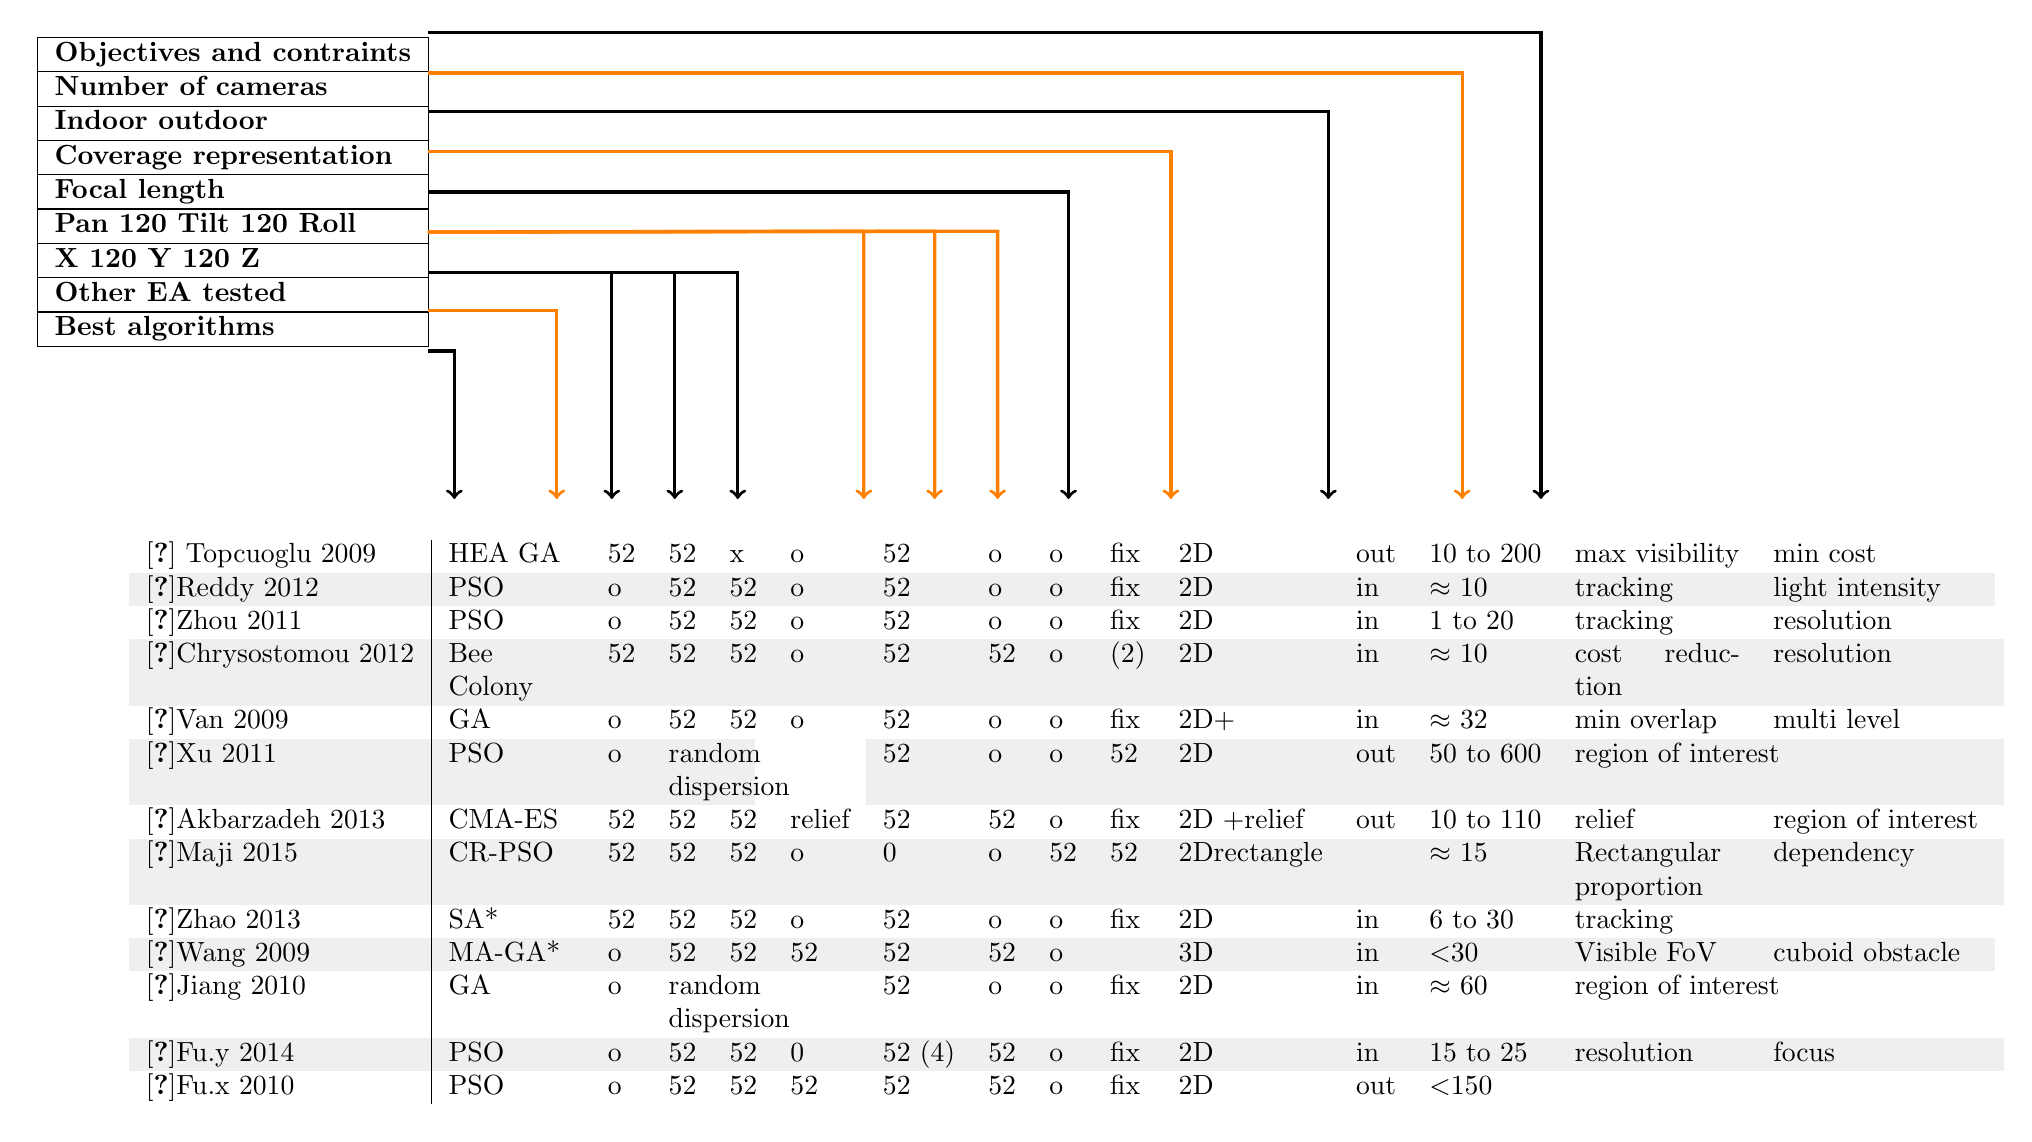
\begin{tikzpicture}[left]
\node (a) at (-0,-0)
{

\begin{tabular}{|l|}
\hline
 % \textbf{Reference} \\ \hline
%   \textbf{Best algorithms}   \\\hline %\vdots
%  \textbf{Other EA  tested}  \\\hline
%   \textbf{X \ding{120} Y \ding{120} Z}\\ \hline
%      \textbf{Pan \ding{120} Tilt \ding{120} Roll }\\ \hline
%         \textbf{Focal length }\\ \hline
%          \textbf{Coverage representation }\\ \hline
%          \textbf{Indoor outdoor }\\ \hline
%           \textbf{Number of cameras }\\ \hline
   \textbf{Objectives and contraints}  \\ \hline
    \textbf{Number of cameras }\\ \hline
    \textbf{Indoor outdoor }\\ \hline
    \textbf{Coverage representation }\\ \hline
    \textbf{Focal length }\\ \hline
    \textbf{Pan \ding{120} Tilt \ding{120} Roll }\\ \hline
    \textbf{X \ding{120} Y \ding{120} Z}\\ \hline 
    \textbf{Other EA  tested}  \\\hline   
    \textbf{Best algorithms}   \\\hline
\end{tabular}
};

\node[yshift=-5.91cm,xshift=22.5cm] (b) at (a.south) 
{
%%               ref  | soluce |EA soluc|x|y|z| pan | tilt |roll | focal |coverage|in out |nmb|
\begin{tabular}{@{} l|p{1.6cm}    l      l l l   l    l      l     l      l         l      l p{2.1cm}p{2.3cm} p{-0.9cm}@{}}
\toprule
\rowcolor[HTML]{F2F2F2} 
%\textbf{ref V2}                                      & \multicolumn{1}{l|}{\cellcolor[HTML]{F2F2F2}\textbf{\begin{tabular}[c]{@{}p{1.59cm}@{}}Best \\ solution\end{tabular}}} & \multicolumn{1}{l|}{\cellcolor[HTML]{F2F2F2}\begin{tabular}[c]{@{}p{0.9cm}@{}}Other\\ EA  \\ solution\end{tabular}} & \multicolumn{1}{l|}{\cellcolor[HTML]{F2F2F2}X} & \multicolumn{1}{l|}{\cellcolor[HTML]{F2F2F2}Y}& \multicolumn{1}{p{0.659cm}|}{\cellcolor[HTML]{F2F2F2}Z}&\multicolumn{1}{l|}{\cellcolor[HTML]{F2F2F2}Pan}& \multicolumn{1}{l|}{\cellcolor[HTML]{F2F2F2}Tilt}& \multicolumn{1}{l|}{\cellcolor[HTML]{F2F2F2}Roll}& \multicolumn{1}{p{1.119cm}|}{\cellcolor[HTML]{F2F2F2}Focal length} & \multicolumn{1}{l|}{\cellcolor[HTML]{F2F2F2}\begin{tabular}[c]{@{}p{1.55cm}@{}}Coverage\\  represen-tation\end{tabular}} & \multicolumn{1}{p{1.56cm}|}{\cellcolor[HTML]{F2F2F2}Indoor outdoor} & \multicolumn{1}{l|}{\cellcolor[HTML]{F2F2F2}\begin{tabular}[c]{@{}p{0.9cm}@{}}Number\\ of \\ cameras\end{tabular}} & \multicolumn{3}{l|}{\cellcolor[HTML]{F2F2F2}\begin{tabular}[c]{@{}l@{}}Secondary \\objectives \\ and contraints\end{tabular}}                                                                \\ \midrule
\rowcolor[HTML]{FFFFFF} 
\multicolumn{1}{l|}{\cellcolor[HTML]{FFFFFF}\cite{101*topcuoglu2009} Topcuoglu  2009} & HEA GA                                                                                                         &  \ding{52}                                                                     &  \ding{52} & x                                              & o                                              &  \ding{52}                                                & o                                                 & o                                                 & fix                                                       & 2D                                                                                                              & out                                                          & 10 to 200                                                                                                 & max visibility & min cost         &                    \\
\rowcolor[HTML]{EFEFEF} 
\multicolumn{1}{l|}{\cellcolor[HTML]{EFEFEF}\cite{33*reddy2012}Reddy 2012}  & PSO                                                                                                            & o                                                                     &  \ding{52} &  \ding{52}                                              & o                                              &  \ding{52}                                                & o                                                 & o                                                 & fix                                                       & 2D                                                                                                              & in                                                           & $\approx$ 10                                                                                              & tracking                                                                                                                    & \multicolumn{2}{l}{\cellcolor[HTML]{EFEFEF}light intensity}      \\
\rowcolor[HTML]{FFFFFF} 
\multicolumn{1}{l|}{\cellcolor[HTML]{FFFFFF}\cite{8*zhou2011}Zhou 2011}   & PSO                                                                                                            & o                                                                     &  \ding{52}                                              &  \ding{52}                                              & o                                              &  \ding{52} & o                                                 & o                                                 & fix                                                       & 2D                                                                                                              & in                                                           & 1 to 20                                                                                                   & tracking                                                                                                                    & resolution                    &                                  \\
\rowcolor[HTML]{EFEFEF} 
\multicolumn{1}{l|}{\cellcolor[HTML]{EFEFEF}\cite{82*chrysostomou2012}Chrysostomou 2012}  & Bee \newline Colony                                                                                                     &  \ding{52}                                                                     &  \ding{52}                                              &  \ding{52}                                              & o                                              &  \ding{52}                                                &  \ding{52}                                                 & o                                                 & (2)                                                  & 2D                                                                                                              & in                                                           & $\approx$ 10                                                                                              & cost reduction                                                                                                              & resolution                    &                                  \\
\rowcolor[HTML]{FFFFFF} 
\multicolumn{1}{l|}{\cellcolor[HTML]{FFFFFF}\cite{83*van2009}Van 2009}  & GA                                                                                                             & o                                                                     &  \ding{52}                                              &  \ding{52}                                              & o                                              &  \ding{52} & o                                                 & o                                                 & fix                                                       & 2D+                                                                                                             & in                                                           & $\approx$ 32                                                                                              & min overlap                                                                                                                 & multi level                   &                                 \\
\rowcolor[HTML]{EFEFEF} 
\multicolumn{1}{l|}{\cellcolor[HTML]{EFEFEF}\cite{84*xu2011}Xu 2011}  & PSO                                                                                                            & o                                                                     & \multicolumn{3}{p{0.89cm}}{\cellcolor[HTML]{EFEFEF}random \newline dispersion}                                                                                    &  \ding{52}                                                & o                                                 & o                                                 &  \ding{52}                                                         & 2D                                                                                                              & out                                                          & 50 to 600                                                                                                 & \multicolumn{2}{l}{\cellcolor[HTML]{EFEFEF}region of interest}                                                                                              &                                 \\
\rowcolor[HTML]{FFFFFF} 
\multicolumn{1}{l|}{\cellcolor[HTML]{FFFFFF}\cite{141*akbarzadeh2013}Akbarzadeh 2013} & CMA-ES                                                                                                         &  \ding{52}                                                                     &  \ding{52}                                              &  \ding{52}                                              & relief                                         &  \ding{52} &  \ding{52}                                                 & o                                                 & fix                                                       & 2D + \newline relief                                                                                                     & out                                                          & 10 to 110                                                                                                 & relief                                                                                                              & \multicolumn{2}{l}{\cellcolor[HTML]{FFFFFF}region of interest}   \\
\rowcolor[HTML]{EFEFEF} 
\multicolumn{1}{l|}{\cellcolor[HTML]{EFEFEF}\cite{143*maji2015}Maji 2015} & CR-PSO                                                                                                         &  \ding{52}                                                                     &  \ding{52}                                              &  \ding{52}                                              & o                                              & 0                                                & o                                                 &  \ding{52}                                                 &  \ding{52}                                                         & 2D \newline rectangle                                                                                                    &                                                              & $\approx$ 15                                                                                              & Rectangular proportion                                                                                                            & dependency                    &         \\
\rowcolor[HTML]{FFFFFF} 
\multicolumn{1}{l|}{\cellcolor[HTML]{FFFFFF}\cite{151*zhao2013}Zhao 2013} & SA*                                                                                                            &  \ding{52}                                                                     &  \ding{52}                                              &  \ding{52}                                              & o                                              &  \ding{52}                                                & o                                                 & o                                                 & fix                                                       & 2D                                                                                                              & in                                                           & 6 to 30                                                                                                   & tracking                                                                                                                    &                               &                                  \\
\rowcolor[HTML]{EFEFEF} 
\multicolumn{1}{l|}{\cellcolor[HTML]{EFEFEF}\cite{152*wang2009}Wang 2009} & MA-GA*                                                                                                         & o                                                                     &  \ding{52}                                              &  \ding{52}                                              &  \ding{52}                                              &  \ding{52}                                                &  \ding{52}                                                 & o                                                 &                                                           & 3D                                                                                                              & in                                                           & \textless30                                                                                               & Visible FoV                                                                                                                 & \multicolumn{2}{l}{\cellcolor[HTML]{EFEFEF}cuboid obstacle}      \\
\rowcolor[HTML]{FFFFFF} 
\multicolumn{1}{l|}{\cellcolor[HTML]{FFFFFF}\cite{165*jiang2010}Jiang 2010} & GA                                                                                                             & o                                                                     & \multicolumn{3}{p{0.659cm}}{\cellcolor[HTML]{FFFFFF}random  \newline dispersion}                                                                                    &  \ding{52}                                                & o                                                 & o                                                 & fix                                                       & 2D                                                                                                              & in                                                           & $\approx$ 60                                                                                              & \multicolumn{2}{l}{\cellcolor[HTML]{FFFFFF}region of interest}                                                                                              &                                  \\
\rowcolor[HTML]{EFEFEF} 
\multicolumn{1}{l|}{\cellcolor[HTML]{EFEFEF}\cite{193*fu2014}Fu.y 2014} & PSO                                                                                                            & o                                                                     &  \ding{52} &  \ding{52} & 0                                              &  \ding{52} (4)                                            &  \ding{52}                                                 & o                                                 & fix                                                       & 2D                                                                                                              & in                                                           & 15 to 25                                                                                                  & resolution                                                                                                                  & focus                         &                                 \\
\rowcolor[HTML]{FFFFFF} 
\multicolumn{1}{l|}{\cellcolor[HTML]{FFFFFF}\cite{194*fu2010}Fu.x 2010} & PSO                                                                                                            & o                                                                     &  \ding{52}                                              &  \ding{52}                                              &  \ding{52}                                              &  \ding{52}                                                &  \ding{52}                                                 & o                                                 & fix                                                       & 2D                                                                                                              & out                                                          & \textless150                                                                                              &                                                                                                                             &                               &                                 
\end{tabular} };
\draw [->,very thick] 		  (-0.135,2.02) -- (14,2.02) -- (14,-3.9); % constraint
\draw [->,very thick][orange] (-0.135,1.51) -- (13,1.51) -- (13,-3.9); % nmb cam
\draw [->,very thick] 		  (-0.135,1.02) -- (11.3,1.02) -- (11.3,-3.9); %in out
\draw [->,very thick][orange] (-0.135,0.51) -- (9.3,0.51) -- (9.3,-3.9);% coverage representation
\draw [->,very thick] 		  (-.135,0.0) -- (8,0) -- (8,-3.9); % focal lengh
\draw [->,very thick][orange] (-.135,-0.51) -- (7.1,-0.5) -- (7.1,-3.9); % roll
\draw [->,very thick][orange] (-.135,-0.51) -- (6.3,-0.5) -- (6.3,-3.9); % tilt
\draw [->,very thick][orange] (-.135,-0.51) -- (5.4,-0.5) -- (5.4,-3.9); % pan
\draw [->,very thick] 		  (-.135,-1.02) -- (3.8,-1.02) -- (3.8,-3.9);  %z
\draw [->,very thick] 		  (-.135,-1.02) -- (3.0,-1.02) -- (3.0,-3.9); % y
\draw [->,very thick]		  (-.135,-1.02) -- (2.2,-1.02) -- (2.2,-3.9); % x
\draw [->,very thick][orange] (-.135,-1.51) -- (1.5,-1.51) -- (1.5,-3.9); %EA tested
\draw [->,very thick] 		  (-.135,-2.02) -- (0.2,-2.02) -- (0.2,-3.9); % best Al
\end{tikzpicture}
\end{table} \label{tab:sum-upEA}
\end{landscape}



%%%%%%%%%%%%%%%%% exemple double  table arrow%%%%%%%%%%%%%%%%%%%%%%%%%%%%%%%%%%%%%

 
%%%%%%%%%%%%%%%%%%%%%%%%%%%%%%%%%%%%%%%%%%%%%%%%%%%%
%\subsection{Field of view}
%
% optical and the occlusion
%
%cover an area with certain amount of sensors. This number of position can be estimate as follow.\\   
%Each camera defined m focusing of optimize the solution and return a acceptable solution.
% 


%####################TODO############################
\section{Coverage path planning}\label{sec:CppLiterattur}

The coverage path planning  has for objective to design  the more efficient path to cover an area. The path has to cover all or  at least most of the area using  the shortest path. \\
The solutions highlighted in the literature until now was about placing numerous cameras or robotics cameras (as PTZ cameras and smart camera) for vast area composed by multiple obstacles.
The solutions proposed until now remains reliable only to monitor a vast area continuously with several cameras. 
The disadvantage of positioning a camera set appears quickly with the cost in computation time. The expensive cost is due to the several cameras and the communication network required to centralize the collected images. All the images must be collected in a real time. \\
In fact, in some applications, the area needs to be controlled periodically. The periodic control of the area does not require an installation for the set of fixed cameras. Until now the installation was composed by a set of immovable cameras unlike the solution presented in section see Section \ref{sec:SolutionBasedonEA} and \ref{sec:NonEAmethod}).
 The periodical control requirement can be illustrated with some example : the cartographies of the area is need just one time and can be completed with one fly over the area roughly bounded as in \citep{66*galceran2013,164*valente2013}, forest fire detection which requires a periodic fly over specific and vast region as in \cite{237*casbeer2006}, the hoovering robots which needs to cover all the room with possibility some on-line computation \citep{218*meiting2007,216*luo2002,215*lee2010,196*yang2004}  and the agriculture.
 About the agriculture application, a UAV needs to fly over the field few times in a year in order to control by photography the hydration, the maturity and anything else of the field as in \citep{164*valente2013,203*zarco2008,63*chao2008,105*long199,167*barrientos2011,177*lelong2008}. %\textbf{revoir les ref et trié un peu}.
For all these applications, the area must be covered but does not need a coverage of all the area instantly and continuously. The solution commonly proposed is the usage of only one sensor mounted on a mobile robot. The Mobile robot need to be adapted to the task and the environment, as flying  \citep{105*long1991}, driving \citep{30*bodor2005,213*roberts2008}, swimming \cite{66*galceran2013}.\\
 The mobile robot with the sensor moves in the space to cover all the area. In this case, the objective is to determine the best path for the mobile robot to cover  the area. The best path is dependent on the constraint of each problem. However, the common point in theses papers is to obtain the shorter path.
The following section is focused on finding the best Coverage Path Planing (CPP) for a sensor mounted on a mobile robot. 
In most cases,  the sensor is a perspective camera. To estimate the best CPP, different algorithms and methodologies have been applied in the literature to solve various problems.

  The following sections are focused on the different algorithms and methodologies applied to optimize the CPP problem. First, the watchman route problem is introduced to highlight the origin of the CPP problem and the relation with the cameras positioning for optimal coverage. In a second time, the more popular solutions are discussed.
 
%hovering robot
% In some case some domestic robots as  the hovering robot   or similar  must also to 213*


%-------------------------------------\\
% Grenzdorffer, G., Engel, A., Teichert, B.: The photogram-metric potential of low-cost UAVs in forestry and agriculture. Int. Arch. Photogram. Rem. Sens. Spatial Inform. Sci.
%31(B3), 1207–1214 (2008) 
%
%Zarco-Tejada, P.J., Berni, J.A., Suarez, L., Fereres, E.: A new era in remote sensing of crops with unmanned robots.
%SPIE Newsroom, pp. 2–4 (2008)
%
%Kazmi, W., Bisgaard, M., Garcia-Ruiz, F., Hansen, K.D.,
%la Cour-Harbo, A.: Adaptive surveying and early treatment
%of crops with a team of autonomous vehicles. In: European
%Conference on Mobile Robots, pp. 253–258 (2011) 


\subsection{AGP  to watchman route problem}\label{sec:WRP}


Before exploring the solutions proposed for the CPP, it is essential to understand the role of the Watchman Route Problem (WRP). The WRP is closely related to the CPP and the WRP has impacted the research about the CPP. 
The following sections are focused on the definition of the WRP, the proposed solutions in order to solve it, and finally, a brief discussion is drawn about the WRP .
 
\subsubsection{Definition of the watchmen route problem }

 \begin{mfigures}[!]
{Watchman route problem answer illustration. }{fig:WRPillust} \centering
\mfigure{width=.4\linewidth}{img/WRPillustration.png}{}{subfig:WRPi}
\hspace{1cm}
\end{mfigures}	
The Watchman Route Problem is introduced for the first time by Chin and Ntafos in 1987 \cite{54*chin1988}. The problem of the WRP can be summarized in one sentence :

\textbf{"How to calculate a shortest route contained inside a polygon such that any points inside this polygon is visible from at least one point of the route?"}.  

The guard has to cover an area represented by a polygon (see the illustration of the problems in Figure \figref{fig:WRPillust}). The guard is considered as \textit{perfect} with no restriction in the field of view (the guard can see at $360^\circ$) and no restriction in the depth field (the guard can see from on extremity of the room to another. The guard can see the opposite wall excepted if an obstacle occludes the view). The guard abilities are directly inspired by the AGP (see \ref{sec:AGP})
The shape of the polygon is primordial and affect greatly the possible solutions and the complexity to solve the WRP.
The WRP problem is by many aspects closely related to the AGP. The AGP (see Section \ref{sec:AGP}) is commonly considered as the root of the WRP.
 In fact, the WRP is not only focused on standing position, but on finding an optimal path. The path has to be optimized to cover all the points which compose the polygon  and the path has to be as shorter as possible.
 
% A common way to build a path with as to cover a polygon can be to search the waypoints  which compose the path. Once the waypoints found the next step is to compute a path passing by all the previously founded waypoints. 
 The next section will introduce the possible methods and algorithms applicable to solve or atleast optimize a solution for a WRP.
 


%polygone impact on the complexity
%AGP -> WRP  

% source : An Approximate Algorithm for Solving the Watchman Route Problem Fajie Li and Reinhard Klette
 
\subsubsection{Solutions} 

The WRP problem can be solved under some conditions. The solutions to solve it are applicable only if the polygon is simple. A polygon is considered as simple, when the boundary of it are composed of continue straight lines that do not intersect between them. To close this definition, it is important to precise the simple polygon does not have any hole (see Figure \figref{fig:simplePoly}). 
 \begin{mfigures}[!]
{Few examples to illustrate the simple polygon shape. }{fig:simplePoly} \centering
\mfigure{width=.4\linewidth}{img/SimplPolygonA.png}{Example of simple polygons.}{subfig:SimplePoly}
\hspace{1cm}
\mfigure{width=.4\linewidth}{img/SimplPolygonB.png}{Example of complex polygons.}{subfig:nonSimplePoly}
\hspace{1cm}
\end{mfigures}	

To solve the WRP, few algorithms were developed. The algorithms proposed in the literature enables  successively better algorithm  to solve the problem. The first interesting algorithm for the WRP with a simple polygon is the early work of Tan et al \cite{234*tan2001}. Tan et al.\citep{234*tan2001}  proposed an algorithm for a fast computation time. The solution proposed works with a simple polygon composed by $n$ vertices and its complexity belongs to polynomial time $O(n^5)$. \\
Others contribution about WRP were then proposed. Dror et al. \cite{233*dror2003} proposed a better time complexity. In fact, in \cite{233*dror2003}, the considered solution with a simple polygon is working in $O(n^3 log n)$ complexity.  The deterministic solution applied is also usable in closely related problems of the WRT as the zoo-keeper problem and safari problem which makes this contribution versatile and generic.
Two other algorithms \citep{234*tan2001,233*dror2003}, are usable only in the case of simple polygons to deliver the optimal solution which is the shortest path for a full room coverage. 

To have a more general solutions for WRP, the proposition lie in having an efficient algorithm working also with complex polygons. A possible solution could be to look for an efficient approximation by optimizing the position of the guards and their respective paths. An efficient approximation means a path acceptably short. In fact the path computed can not be certified as the "best path" but only as the shorter found.

Several efficient approximations have been proposed such as in \citep{235*faigl2010} and \citep{53*packer2008}. 

In Packer \citep{53*packer2008},  the algorithm proposed is based on splitting the problem into two sub-problems. The first sub-problem consider the search of a set of points which can be good enough to cover all the area despite a restricted visibility range. These points are called waypoints.  
Once the set of waypoints to cover all the polygons are found, the second sub-problem consider the creation of a path passing by all these points. 
 This second sub-problem is similar to a classic Travelling Salesman Problem (TSP). The TSP tries to answer the questions asked by a travelling salesman "\textbf{What is the shortest path passing by each city only one time and return to the starting city?}".
  In the TSP, the cities are the nodes on the interconnected map and the roads are the connections between them. The TSP is a well known NP-hard and NP-complete problem when applied in  some conditions, as described in \citep{236*karp1972}. \\ 
Finally the solution used for the TSP can be applied for the second sub-problem of WRT.
Subsequently, TSP can be applied for the second sub-problem of WRT solution proposed by Packer \citep{53*packer2008}.

%a similar method than the one proposed by faigl in [235*] has been proposed to approximate the shorter path as possible. To approximate the shorter path the problem of WRP is also split in two sub-problem. The first sub-problem is considered as similar then the AGP and use the method form AGP to find the waypoints. The second sub-problem is also compared as TSP.

In Faigl  \citep{235*faigl2010}  a similar method to the one proposed by Packer \citep{53*packer2008} has been proposed to approximate the shorter path. The problem is also split into two sub-problems. The first is to optimize the position of the waypoints and the second is to schedule the position in order to create a path planning (directly inspired by the TSP). 
%the algorithm proposed is based on splitting the problem into two sub-problems. The first sub-problem is to find a set of point with can be good enough to cover all the area despite a restricted visibility range. These points are called waypoints for the following sections. 
 Furthermore, the solution proposed by Faigl in \citep{235*faigl2010} is applicable to a watchman with a restricted visibility range i.e. equivalent to a $360^\circ$ field of view with a \textit{restricted depth of field}. This restriction affects greatly the waypoints positioning. Due to this constraint, more waypoints needs to be placed to cover an area.
 Once the set of waypoints for the polygon coverage is found, the second sub-problem is to create a path passing by all these waypoints.  The algorithms proposed  to perform such task are also inspired by the solution given for the optimization of the TSP.
 %This second sub-problem is similar then a classic Travelling Salesman Problem (TSP). The TSP  try to answer the question ask by a travelling salesman "What is the shortest path passing by each city only one time and return to the starting city?". In the TSP, the city are the node on the interconnected map with the road as the connexion. The TSP is well known as NP-hard and NP-complete in some condition as described in [236*]. \\ 
%Finally the solution used for the TSP can be applied for the second sub-problem of WRT.
% The TSP and the algorithms proposed to optimize it are discussed more in detail later \ref{par:TSPPathPlan} \\
%In Packer [53*] similar solution than the one proposed by faigl in [235*] has been proposed to approximate the shorter path as possible. To approximate the shorter path the problem of WRP is also split in two sub-problem. The first sub-problem is considered as similar then the AGP and use the method form AGP to find the waypoints position. When the  waypoints are placed in the polygon the second sub-problem which is to schedule the waypoints to have a shorter path as possible. 



%from https://link.springer.com/content/pdf/10.1007%2F978-3-642-31155-0.pdf
%compexity $O(n^4 log n)$ :\\
%Dror, M., Efrat, A., Lubiw, A., Mitchell, J.S.B.: Touring a sequence of polygons.
%In: Proc. 35th Symposium on Theory of Computing, pp. 473–482 (2003)\\
%Tan, X.: Fast computation of shortest watchman routes in simple polygons. Information Processing Letters 77(1), 27–33 (2001) \\ 

%linear approximation :  Tan, X.: A linear-time 2-approximation algorithm for the watchman route problem for simple polygons. Theoretical Computer Science 384(1), 92–103 (2007)

%Polygons with holes the problem is NP-hard : 54*\\
 %  Dumitrescu, A., T oth, C.D.:Watchman tours for polygons with holes. Computational Geometry: Theory and Applications  (2012)

 %An $O (log n)-approximation$ for Rectilinear polygons are also known as orthogonal polygons.:Mata, C.S., Mitchell, J.S.B.: Approximation algorithms for geometric tour and network design problems. In: Proc. 11th Symposium on Computational Geometry, pp. 360–369 (1995)

\subsubsection{Limit and consequences}

The methods proposed to solve the WRP are really interesting and gives a good solution in some specific conditions. These conditions make his methods special cases.
 In fact the optimal solution, i.e. the shortest path which covers all the area (polygon), are usable only if the polygons observe some rules. The polygon must be simple and take into account the guard ability (no viewing constraints).  \\
When the polygon is more complex, the optimal solution cannot be reached. The methods applied to solve the WRP for complex area are promising. Especially the problem splitting into sub-problems. Despite this interesting aspect, the solutions proposed are most of the time limited due to the area representation. This representation associated to the geometric methodologies to find the waypoints gives a crucial importance to the number of vertices inducing also the number of cameras. \\
A large  number of vertices imply  consequently that the first sub-problem may be difficult and time-consuming to solve.
Consequently this method is not the more appropriate for vast and complex outdoor areas which would require  numerous vertices to describe.
 The biggest limit of the WRP is the ability of the watchmen. Indeed, in the original problem, the watchmen are considered having a perfect visibility. The solution proposed solving the WRP are not usable with the accumulation of new visibility constraints. 
In Faigl \citep{235*faigl2010}, the WRP started to be extended by adding a constraint on the visibility. In this condition the problem is slightly modified to shift from self-organizing map to  coverage path planning. But despite this addition of a restricted  depth of field, the proposed solution based on geometric heuristic do not allows the accumulation of more constraints.

The AGP then WRP extensively impacted the vision, the design of cameras coverage problem  and coverage path planning field.  Among the solutions discussed in the previous section, numerous articles are based and/or refers to the AGP and WRP. Our work is consequently inspired by those formulations and will propose to extend it.



 


%tout comme l'agp a était une source d'inspiration pour  le positionnement de camera  le wmp est lui aussi une source d'inspiration pour  le cpp 
%The CPP 
%The origin of CPP can be found on the Watch Men Problem (WMP). The next
%
%The Watch Men Problem (WMP) is directly derived form the AGP. 
%
%As the importance of AGP for the problem of camera positioning  the Watch men problem 
%53* parcker eli :  propose a solution  to solve the watchmen problem based on the result optianined by the AGP \\ 
%54* Chin : complexity proof of NP-hard  for the watchmen problem by reduction of TSP + article fondateur
%

\subsection{CPP solutions}



To optimize the CPP problems many solutions were proposed. The different algorithms and methodologies proposed are discussed in the following sections. The methodologies proposed can be organized in several branches. 
The most important branch to optimize the CPP corresponds to the usage of sweep associate to a cellular decomposition.
%60* =  une découpe en zone  rectangle et utilisation  de la triangulation pour le positionment de waypoint  puit tsp.
%
%217*= utilisation du GA  pour la conexion entre polygone simple (1er étape découpe de la zone  en  polygone en fonction des obstacle - 2e  crée un graphe qui  reli les différant sous partie ( polygone) GA  -3 choisir le sweep le plus )
%
%61* 62*= floor planning

\subsubsection{Cellular decomposition and sweep} \label{sec:CPPcellDecompSol}
\begin{mfigures}[!]{Illustration  of  simple cell decomposition with sweep.}{fig:CellDecp} \centering
\mfigure{width=.4\linewidth}{img/CellDecop.png}{}{}

\end{mfigures}	
To solve the CPP problem, the most common solution is considered to be the cellular decomposition. The cellular decomposition is by some aspects inspired by the methodologies presented in the WRP.
To recall one of the interesting solution for the WRP, the methodology starts by splitting the problem in two sub-problems and optimize those independently. The first sub-problem solve the search of the best waypoints and the second sub-problem corresponds to finding the shortest path passing by all the waypoints (like the TSP).
 The Cellular decomposition also split the problem of CPP in two sub-problems. The first sub-problem is focus on the decomposition of the complex area in several cells. Each cell has to be a simple polygon (basically a rectangle or latter any quadrilateral polygon). Inside each cell a sweeping has be applied in order to cover all the area (see Figure \figref{fig:CellDecp}). The second sub-problem is to find the path which can connect each simple polygon. The problem has to take in account, the sweep start and end to find the global optimized shorter path. Where the global optimized shorter path take in account the sweep trajectory of each simple polygon and the path between the simple polygons.
 
 Finally the cellular decomposition is made by decomposing the complex area, choosing the appropriate sweep and finding the shortest path to connect the cells. 
 
 \paragraph*{Decomposition}\label{par:decomposition}

 The decomposition in cells has for objective to split a complex area in several sub-areas. Each sub-area has to be simple in term of shape in order to apply a sweep. 
Since the 90s, numerous algorithms have been developed for the cellular decomposition. Among the algorithms for cellular decomposition, 3 types of decomposition were deduced as shown in the survey of Choset  \cite{214*choset2001} and  Galceran and al \cite{66*galceran2013}. 
\begin{itemize}
	\item Approximate: 
		An approximate decomposition is based on discretization of the area. The free space of the area is represented by a set of cases (grid). Each case of the grid has to be covered by a mobile robot. A case is considered completely covered if the robot is on the associated position. Which means that the frequency of the grid is defined by the covered area of the mobile robot. 
		The approximate decomposition by cases is convenient to describe the area but is greatly limited due to the low sampling frequency of the gird and the limited amount of possible trajectories.\\
	 
	\item Semi approximate: 
	 \begin{mfigures}[!]
{Illustration of a semi approximate decomposition outcome from the survey  of Choset \citep{214*choset2001}. The 4 figures illustrates the trajectory of the robot over the time.}{fig:choset214SemiAprox} \centering
\mfigure{width=.95\linewidth}{img/Choset214SemiDecomp.png}{}{subfig:WRPi}
\hspace{1cm}
\end{mfigures}	
 The semi approximate decomposition is partly based on the discretization of the space. The idea is to create a set of large cells. The width of the cells is fixed and the height is relative to the area boundaries (see in \citep{214*choset2001}). 
	 The semi approximate cell decomposition allows to have cells with two parallel sides with a fixed size (right and left) and  the  two other sides adapted to the boundaries (up and down. See the illustration  of a semi approximation in Figure \figref{fig:choset214SemiAprox}).  The width  of  the cells are chosen accordingly to half of the focal length of the camera mounted on the mobile robot. The area is covered by following the boundaries of the cells with sweep to cover cells  after cells.
	 The advantage of the semi approximate decomposition is the ease to describe a vast area and the low computation time required. Additionally, this decomposition can be made on-line by the robot and do not requires a high level of knowledge of the area. 
	 The disadvantage is the non-optimization of path due to the cells decomposition. The simplicity  of this decomposition  can generate case where the robot have to cover many times the same place. The semi approximate cellular decomposition do not allow to have a well optimized path planning. \\
	 
	 %%%%% add fig from238* fig8 to --> from214
	\item Exact cellular decomposition: 
	The exact cellular decomposition describe the area by creating juxtaposed geometrical regions. The size of the regions (or cells) are not depending on the robot ability contrarily to the previous decomposition. The large size of the cells allows the  mobile robot to do back and forth motion to cover all the cells (also called sweep as in Figure \figref{fig:sweepSpiral}).  The cells have to be ordered to conserve an efficient and short path going through all the cells. 
The global path distance have to be reduced by an appropriation of the path passing through cells.
	The exact cellular decomposition became popular and numerous algorithms have been proposed. The proposed algorithms  can be a faster decomposition or a deduction of more appropriate shape depending on the basic rectangular cells. 
	Among the numerous exact cellular decomposition propositions: the trapezoidal decomposition for its simplicity and historic importance, the Boustrophedon decomposition  and  Morse-based Cellular Decomposition can be cited for their importance in the construction of other exact cellular decomposition. These algorithms and other are clearly summarized in the survey of Carreras and Galceran \citep{66*galceran2013}. 
	The exact cellular decomposition has been still studied since the survey of  Carreras and Galceran  \citep{66*galceran2013} and upgraded, as in \cite{144*torres2016}, proposing a decomposition for concave or multiple polygons.
	
\end{itemize}




% survey = 66* 214*
% CPP experimentation (164* 167*)
% 
%119* 214* 215* 146*  144* 164* 167* 190*=cellule decomposition \\ 

 
 \paragraph*{Sweeps} \label{par:sweep}
	The back and forth or sweep is an essential element of the CPP by cellular decomposition. The sweep has to cover the entirety of the cells. The cells are splitting the area in relatively simple polygons (as shown in the paragraph \ref{par:decomposition} and  the Figure \figref{fig:CellDecp}). The sweep needs to be adapted to the shape of the cells and also must start and finish in a appropriate position taking into consideration the path to the next cells.
	For that the starting point and the ending point of the sweep are crucial for the global path planning.
	In Torres et al. \cite{144*torres2016},  the sweep is function of a direction and can go clockwise or counter-clockwise to have a start and end in the appropriate position for the transition. 
	 This enables to have 8 different applicable sweeps at each cells depending on the most appropriate start and finish; according to the computed path. The sweeps are adapted depending on : 
	 \begin{itemize}
	 \item The turn sides ( clockwise or counter-clockwise)
	 \item The directions (horizontal or vertical)
	 \item The finishing  positions (start and stop from the same side or opposite side)
\end{itemize}	
	 The sweep can be also alternatively switched for a spiral as proposed in Jimenez et al. \citep{217*jimenez2007}. The proposed sweep and spiral  are adaptable depending on the context. The sweep can have two directions and for the spiral two turn sides (clockwise or counter-clockwise).  The different sweeps and spirals are illustrated in the Figure \figref{fig:sweepSpiral}. 
	  \begin{mfigures}[!]{Illustration of the different sweeps and spirals.}{fig:sweepSpiral} \centering
\mfigure{width=.55\linewidth}{img/SweepSpiral.png}{}{}
\end{mfigures} 

	To have an adapted sweep, the footprint has to be defined depending on the camera ability and the objectives. In \cite{144*torres2016}, the size of the sweep is dependent on the area covered by a camera and a considered sufficient amount of overlaps for the 3D reconstruction (see also\citep{191*di2016}). In Li et al.  \citep{146*li2011}, the footprint of the camera with a small pan is considered. Due to the pan, the camera projection is not a rectangle but a trapezoid. Consequently the sweep size is adapted by taking the larger side of the trapezoid for the sweep dimension.
	Also for the grid decomposition, the sweep size is directly related to the coverage ability of the mobile robot (as example in \citep{215*lee2010,195*choi2009}).  % also 216*+48  215*  195* +55 218*+12  use a sensing camera at the front).
	
	One extra element necessary for the sweep can be in some cases the external element such as the wind. In \citep{215*lee2010,190*hsu2014},  %!![190*] !! 
	the external condition are taken into account in the cost function and it influence the sweep.
	
	
	To summarizes the sweeps requires to be adapted to the area and the relation between cells. To choose the appropriate sweeps the following element have to be considered:
	\begin{itemize}
		\item The size of sweep  have to be defined depending on the ability of the camera (footprint size).
		\item The direction (horizontal or vertical).
		\item The  starting and finishing  position (start and stop from the same side or opposite side)
	\end{itemize}
To  obtain the more appropriate sweep, it is primordial to know before the cells scheduling. The cells scheduling are a crucial part of the path planning.

	% The foot print, 
	 %the type of sweep ( sweep or spiral), the direction (horizontal or vertical), the finishing  position (start and stop form the same side or opposite side) the size of the footprint has to be defined depending then the ability of the camera. 
	
	%215* 190* generic cost depending then external condition  and  using spiral or sweep
	 
	 %144*  size to the sweep adapted  depending then the footprint of the camera on the ground floor  with propose lot of overlap useful for the 3D reconstruction.  the sweep  is function then a direction  and can go  clockwise or counter-clockwise to have  a start and end in the appropriate position for the transition. 
	 %This allow to have 8 different sweep applicable at each cell depending then the more apropriate start and finish depending  then the turn side ( clockwise or counter-clockwise), the direction (horizontal or vertical)  and the finishing ( start and stop form the same side or opposite side).  
	% 217*  propose  sweep and spiral with  different direction  for the sweep and two turn side for the  spiral

	%195* spiral sweeping for on-line coverage (for hoover application)
	 
%	209* comparative between cellular decomposition with sweep and a global spiral on the complex shape. (master these)
	
	
    
 
 %décompostion celulurai avec étude sur le remplisage sweep ou  spyrale pour  des zone concave our convex 
%Ost, G.: Search Path Generation with UAV Applications Using Approximate Convex Decomposition, Masters Thesis. Linkopings universitet, Sweden (2012)

 
 \paragraph*{Path planning} \label{par:TSPPathPlan}
 
The aim of the path planning is to find the short path going through all the cells. Finding the best path planning passing by all the waypoints or in this case all the cells, is a complex problem  which can be formulated as a TSP. The path planning became even more complex in the case of exact cellular decomposition or for any decomposition which requires a sweeping inside each cells. Indeed, in this case, the goal is to have the shortest path planning with taking into account each sweep and transition between cells. In the previous paragraph \ref{par:sweep}, the different sweeps and spirals have been detailed. The start and the end of the sweep are the crucial elements to consider during the path planning computation.
 Obviously, to find the best scheduling between each cells, the algorithm induces by the TSP are commonly used.     
 
 When the area is decomposed in cells, the goal is to schedule the right-of-way from one cell to another in order to create an efficient path. The scheduling of the cells can be optimized by using the paradigm of TSP with the same algorithms to have an acceptable path planning. 
The TSP is a well known problem and is deeply studied from long time ago. First is essential  to remember the TSP is an NP-complete and NP-hard problem as prooved in Karp in \cite{236*karp1972}. 

To optimize the TSP, numerous algorithms have been tested and some of them have been specially applied to schedule the cells to have the shortest path. In  An et al. \cite{60*an2013}, two algorithms were tested before developping a third. The algorithms used are based on branch and bound. The algorithm developed in \cite{60*an2013} is called Novel Previous-Next Waypoints Coverage Constraint (PNWCC). The algorithms presented in \cite{60*an2013} proposes at same time a schedule of each cells as well as a smooth trajectory without sharp edges usable for non holonomic driving robots. 

In the survey of Carreras et Galceran \citep{66*galceran2013}, the solutions proposed to solve the TSP are asked to compute an exhaustive walk trough the adjacency graph. These solutions are workable only for computingg small adjacency graph. The GA is popular to optimize the TSP and is commonly used to evaluate the influence of parameters as in \citep{68*muhlenbein1989} \citep{80*serpell2010}. About the CPP problem, the GA is also used to optimize the TSP part as in Jimenez et al. \citep{217*jimenez2007}, where the GA is applied to find an optimized schedule retrospectively of an exact cellular decomposition of a complex polygon. \\
The GA is announced to be appropriated to obtain an optimized solution for the TSP. 
In some situations, a  TSP is not realistic and some external constraints can be added such as the wind effect, turbulence, or holonomy constraint as in \citep{56*davies2006,102*ware2016,66*galceran2013}). The addition of external constraints may leads to more complex scheduling  of the cells. 
 
 
%236* proof of NP complet and NP-hard

%60* use of TSP = any TSP algorithm can be used  as the branch and bound algorithm. or best choice is to use  the Hearest Neighbor algorithm  and finally propose a Novel PNWCC solution with propose a path without  sharp edges usable for non holonomic driving robots.
%66* TSP  solver with a  several methode. 
%217* use of TSP  solved with GA (CPP)217*  GA  for the TSP

%102* TSP with external constraint (wind)
 
%68* asyncorne parallel GA for TSP
%80* GA mutation rate for TSP 
%139* GA config for TSP
%172* TSP GA   Use of GA multi goal for  schedule the charge on  m machine and n job  

%XX 56* evitement d'obstacle et trachectioire 
%XXX 214* reference of the problem 
%XXX 164*  use TSP 


%%%%%\subsubsection{Other solution for CPP}
%%%%%	216* 218* 215* 196*= robot roulant hoover \\
%%%%%	
%%%%%	191* 190* 211* 212* = low enregie cpp\\
%
%In choset et al 214*  some heuristic and randomized solution has been presented.    
%one of the basic heuristic is to follow the boundary of the area to cover. (R.A. Brooks, A robust layered control system for a mobile robot, IEEE J. Robotics Autom. (1986)   et
%  E. Gat and G. Dorais, Robot navigation by conditional sequencing, in: Proc. IEEE Int. Conf. on
%Robotics and Automation, San Diego, CA (May 1994) pp. 1293–1299. )
%
%	\begin{itemize}
%	\item Liu, Y., Lin, X., Zhu, S.: Combined coverage path planning for autonomous cleaning robots in unstructured environments. In: Proc. World Congress on Intelligent Control and Autom., pp. 8271–8276 (2008) 
%
%	\item Luo, C., Yang, S.X.: A bioinspired neural network for
%real-time concurrent map building and complete coverage robot navigation in unknown environments. IEEE
%Trans. Neural Netw. 19(7), 1279–1298 (2008) == PDF TNN2008  cite 132  neural network pour  robot aspirateur  avec construction de la map  et complet couverture  
%	
%	\item Oh, J.S., Choi, Y.H., Park, J.B., Zheng, Y.F.: Complete coverage navigation of cleaning robots using
%triangular-cell-based map. IEEE Trans. Ind. Electron. 51(3), 718–726 (2004) == pdf navigation-robot.pdf   robot roulant construction de son univer ajout de direction possible
%
%	\item 214* = propose 2 heuristic  et randomize 
%	\end{itemize}
	
	
%	177*= multi spectral\\
%	119* 214* 215* 146* 66* 144* 164* 167* 190*=cellule decomposition \\
%	146* 147* = optimization de trajectoire local cpp\\
%	196* =neural Network \\
%	195* 189*= ???
%
%%\subsubsection{ ??sensor positioned in electronic circuit ??}
%%\subsection{Robot application}
%	%\subsubsection{hover robot}
%	%\subsubsection{submarine}
%	
%	
%	!!!!!!!!!!!!!!!!!!!!!!resource!!!!!!!!!!!!!!!!!!!!!!!!!!!!\\ 
%	from 190
%
%\subparagraph{Probelm du CPP par Genetic Algo GA }	
%\begin{itemize}
%	\item Jimenez, P.A., Shirnzadeh, B., Nicholson, A., Alici, G.: Optimal area covering using genetic algorithms. In: Proc. IEEE/ASME Int. Conf. Advanced Intelligent Mechatronics, pp. 1–5 (2007)
%	
%	\item Wang, M., Tan, S., Yan, L.: Complete coverage path planning of wall-cleaning robot using visual sensor. In: Proc. Int. Conf. Electronic Measurement and
%Instruments, pp. 159–164 (2007)
%
%	\item Zhang, G., Ferrari, S., Qian, M.: An information
%roadmap method for robotic sensor path planning. J. Intell. Robot. Syst. 56(1–2), 69–98 (2009)
%	\end{itemize}
%
%
%\subparagraph{CPP  résolution par  neural Network pour certain une gestion dinamique de obstacle  }	
%\begin{itemize}
%	\item Lee, T.K., Baek, S.H., Oh, S.Y., Choi, Y.H.: Complete coverage algorithm based on linked smooth spiral paths for mobile robots. In: Proc. Int. Conf. Control, Automation, Robotics and Vision, pp. 609–614 (2010)
%
%	
%	\item Yang, S.X., Luo, C.: A neural network approach to complete coverage path planning. IEEE Trans. Syst. Man Cybern. 34(1), 718–725 (2004)
%
%
%
%	\item Luo, C., Yang, S.X., Stacey, D.A., Jofriet, J.C.: A solution to vicinity problem of obstacles in complete coverage path planning. In: Proc. IEEE Int. Conf. Robotics
%and Automation, pp. 612–617 (2002)
%
%\item Qiu, X., Song, J., Zhang, X., Liu, S.: A complete coverage path planning method for mobile robot in uncertain environments. In: Proc. World Congress on
%Intelligent Control and Automation, pp. 8892–8896 (2006)
%
%
%\item Qiu, X., Liu, S., Yang, S.X.: A rolling method for 
%complete coverage path planning in uncertain environments. In: Proc. IEEE Int. Conf. Robotics and
%Biomimetics, pp. 146–151 (2004)
%
%\item Luo, C., Yang, S.X., Stacey, D.A.: Real-time path planning with deadlock avoidance of multiple cleaning
%robots. In: Proc. IEEE Int. Conf. Robotics and Automation, pp. 4080–4085 (2003) 
%
%	\end{itemize}
%
%\subparagraph{survey  sur la décomposition  linaire }
%	\begin{itemize}
%	\item Choset, H.: Coverage for robotics-a survey of recent results. Ann. Math. Artif. Intell. 31, 113–126 (2001)
%	
%	\end{itemize}
%	
%	\paragraph{66*  points clé}
%	coverage path planning in the 3D space (UAV and Subamrine)\\ 
%	cellular decomposition :  requantangle cellul  ;  trapezoidal decomposition ; Boustrophedon Decomposition; Morse-based Cellular Decomposition ; online Morse-based Boustrophedon Decomposition ; Landmark-based Topological; slice Decomposition ;On-line Topological Coverage Algorithm ;Contact Sensor-based Coverage of Rectilinear Environments;Grid-based Methods;Grid-based Coverage using the Wavefront Algorithm;Neural Network-based Coverage on Grid Maps
%Coverage 
%		\paragraph{214* choset}
%		heurisitc and randomized approche :  propose a solution  on multi robot repultion system to spread the  robot  in the space and  use   a random motion  as strategie to explore the area[5,27]. \\(T. Balch and R.C. Arkin, Communication in reactive multiagent robotic systems, Autonom. Robots 1995) , unknown obstacles of arbitrary shape, Algorithmica 2 (1987) 403–430. ;:;\\ D. MacKenzie and T. Balch, Making a clean sweep: Behavior based vacuuming, in: AAAI Fall Symposium, Instationating Real-World Agents (1996). )
%		
%		\paragraph{Semi-approximate}
%		Hert and Lumelsky : propose a system based on cell decomposition  and   boundary folowing 
%		
%		\paragraph{multi robots}
		
		\subsubsection{Other solutions}
		
		Among the algorithms developed for the CPP, some interesting methods have to be studied.		
		Some algorithms has been discussed in Choset \cite{214*choset2001} as approximate solution (see Section \ref{par:decomposition}). 
		
%	!!!	Despite this classification the decomposition of the area is not the really effective and the algorithms used must be highlight. Among it the solution based on regular grid discretization which this  comparatively to cellular decomposition high sampling frequency. As discussed earlier in this case the cell decomposition is made based on the coverage ability of the  mobile robots as  well detailed in \citep{218*meiting2007}.
%		Thanks to this relatively fine grid decomposition the number of case and the regularity of its the TSP paradigm is not the more appropriate and other solution may used to optimize the path planing of the mobile robots.
%		This solution is relatively popular for the plan the hoover robot path as in  \citep{216*luo2002,196*yang2004,215*lee2010,218*meiting2007}.
%		The idea is to have an algorithms which not tried to optimize globally the path planning but have an adapted local decision with maximize the global path plan. !!
		 The approximate cellular decomposition was briefly approached in the previous Section \ref{par:decomposition}. The approximate cellular decomposition was considered  not interesting due to the low sampling frequency of the grid. Conceptually, the works of \citep{216*luo2002,196*yang2004,215*lee2010} are going further by using a higher sampling frequency of the area to cover. The  solution based on regular grid discretization may be compared to  approximated cellular decomposition with a high sampling frequency as in \citep{218*meiting2007}.
		  Due to the relatively fine grid decomposition which engender an increased size of the cases number, the algorithms to optimize the path  passing by all the cases of the grid has to be adapted . Consequently,  new navigation strategy has been developed. 
		
		In Luo et al. \citep{216*luo2002}, the goal is to have a complete coverage by visiting all the cases of a grid. To visit all the cases of the grid, a neural-neighborhood analysis and neural dynamic programming approaches are adapted to have an efficient CPP for the robots. In Simon et Luo \citep{196*yang2004}, they proposes an similar method with a neural network solution for dynamic and non planar area.
		
		The work of Lee et al. \cite{215*lee2010} proposes another solution based on smooth spiral path. The idea is to propose to follow the boundaries of the room in order to fully cover and use a smoothed spiral to cover the area. The solution proposed is compared to other methods. The main advantage of these method is the on-line ability and the smoothed trajectory (see also \citep{195*choi2009}).
		
		Before to conclude about some of the algorithms usable to optimize the coverage path planning the more elementary has to be discussed. In fact,  among the algorithms proposed until here the full random was not discussed. 
		In Liu et al. \cite{242*liu2008}, a really basic method is developed to cover an area with a mobile robot (hover robot) for on-line path planning in a dynamic environment. The algorithm proposed is based on random directions. The basic idea is to move forward until the detection of an obstacle (ultrasonic or bumper). When an obstacle is detected, the robot turns randomly. This solution is really basic and is based on the idea saying that if the room is not too big or not specially complex, with enough time, the mobile robot will cover all. Obviously this solution is not optimized and not suitable in many cases. 
		
		


		
		%	177*= multi spectral\\
%	119* 214* 215* 146* 66* 144* 164* 167* 190*=cellule decomposition \\
%	146* 147* = optimization de trajectoire local cpp\\
%	196* =neural Network \\
%	195* 189*= ???
%%%%%	216* 218* 215* 196*= robot roulant hoover \\
%%%%%	
%%%%%	191* 190* 211* 212* = low enregie cpp\\


%\subparagraph{CPP  résolution par  neural Network pour certain une gestion dinamique de obstacle  }	
%\begin{itemize}
%	\item Lee, T.K., Baek, S.H., Oh, S.Y., Choi, Y.H.: Complete coverage algorithm based on linked smooth spiral paths for mobile robots. In: Proc. Int. Conf. Control, Automation, Robotics and Vision, pp. 609–614 (2010)
%
%	
%	\item Yang, S.X., Luo, C.: A neural network approach to complete coverage path planning. IEEE Trans. Syst. Man Cybern. 34(1), 718–725 (2004)
%
%
%
%	\item Luo, C., Yang, S.X., Stacey, D.A., Jofriet, J.C.: A solution to vicinity problem of obstacles in complete coverage path planning. In: Proc. IEEE Int. Conf. Robotics
%and Automation, pp. 612–617 (2002)
%
%\item Qiu, X., Song, J., Zhang, X., Liu, S.: A complete coverage path planning method for mobile robot in uncertain environments. In: Proc. World Congress on
%Intelligent Control and Automation, pp. 8892–8896 (2006)
%
%
%\item Qiu, X., Liu, S., Yang, S.X.: A rolling method for 
%complete coverage path planning in uncertain environments. In: Proc. IEEE Int. Conf. Robotics and
%Biomimetics, pp. 146–151 (2004)
%
%\item Luo, C., Yang, S.X., Stacey, D.A.: Real-time path planning with deadlock avoidance of multiple cleaning
%robots. In: Proc. IEEE Int. Conf. Robotics and Automation, pp. 4080–4085 (2003) 
%
%	\end{itemize}